\section{Resultados}
\subsection{Servidor unak.is}
\begin{figure}[H]
  \centering
    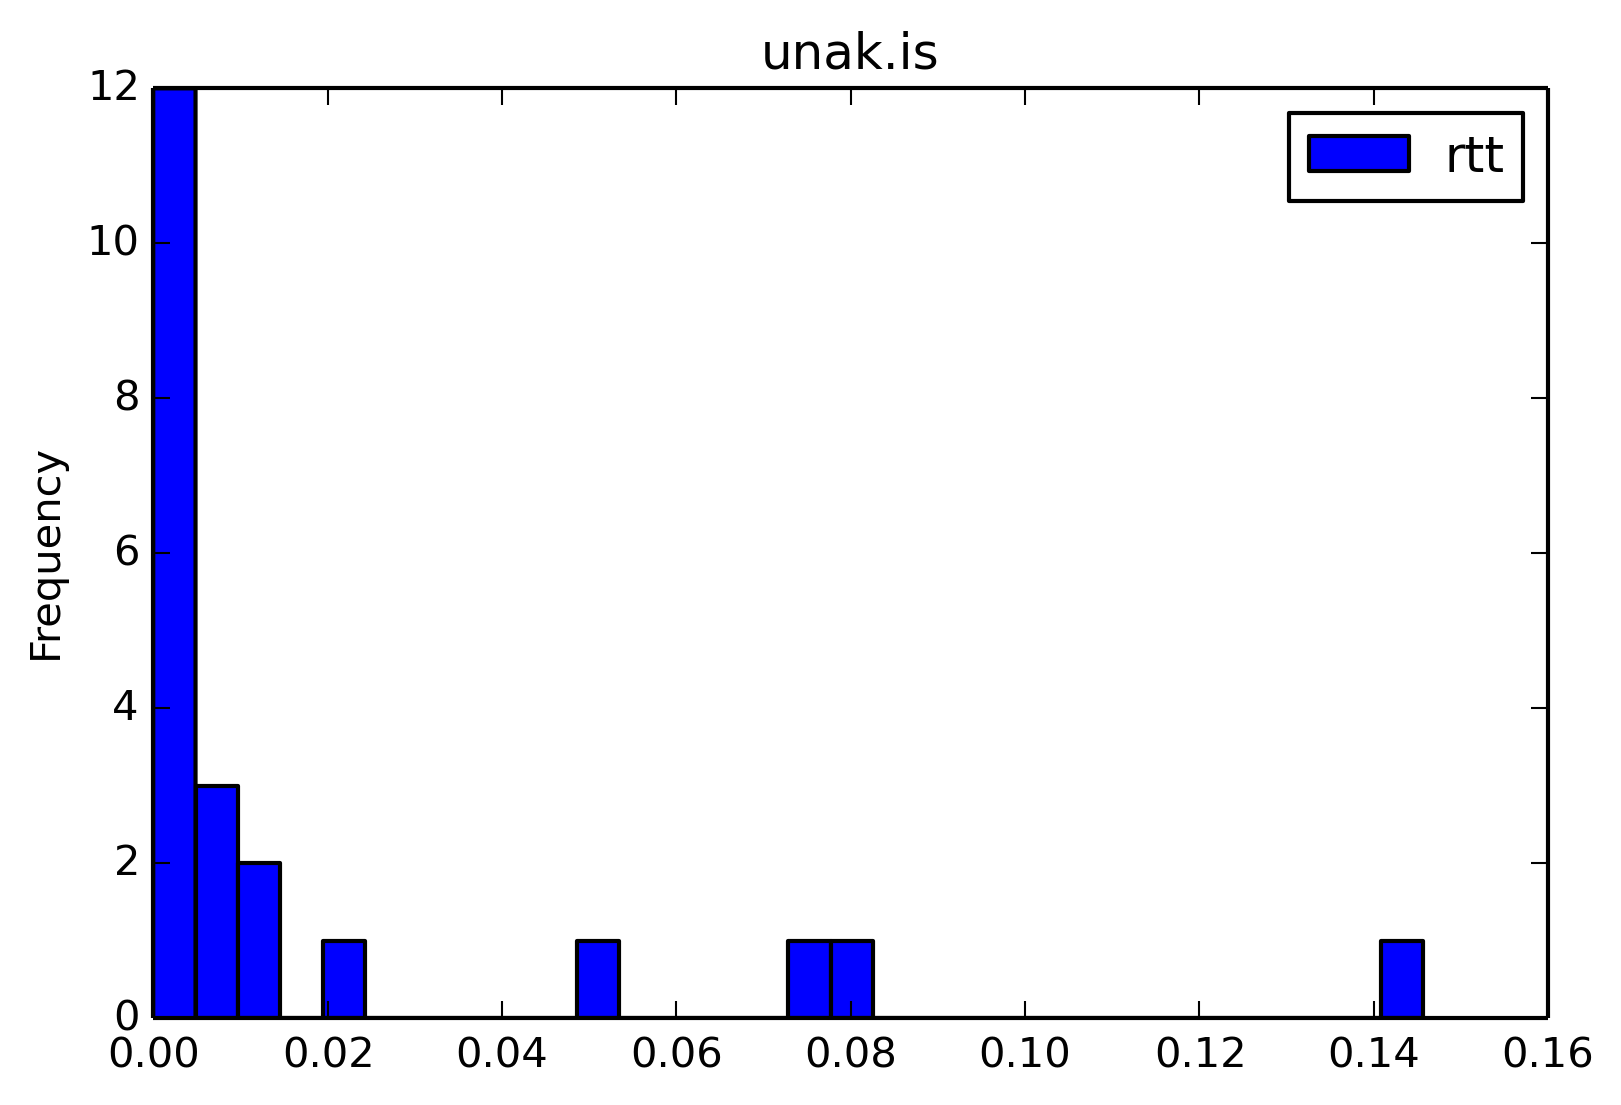
\includegraphics[width=0.45\textwidth]{histogramas_rtt/unak-is.png}
  \caption{RTT entre saltos}
  \label{entropia-s}
\end{figure}

\begin{figure}[H]
  \centering
    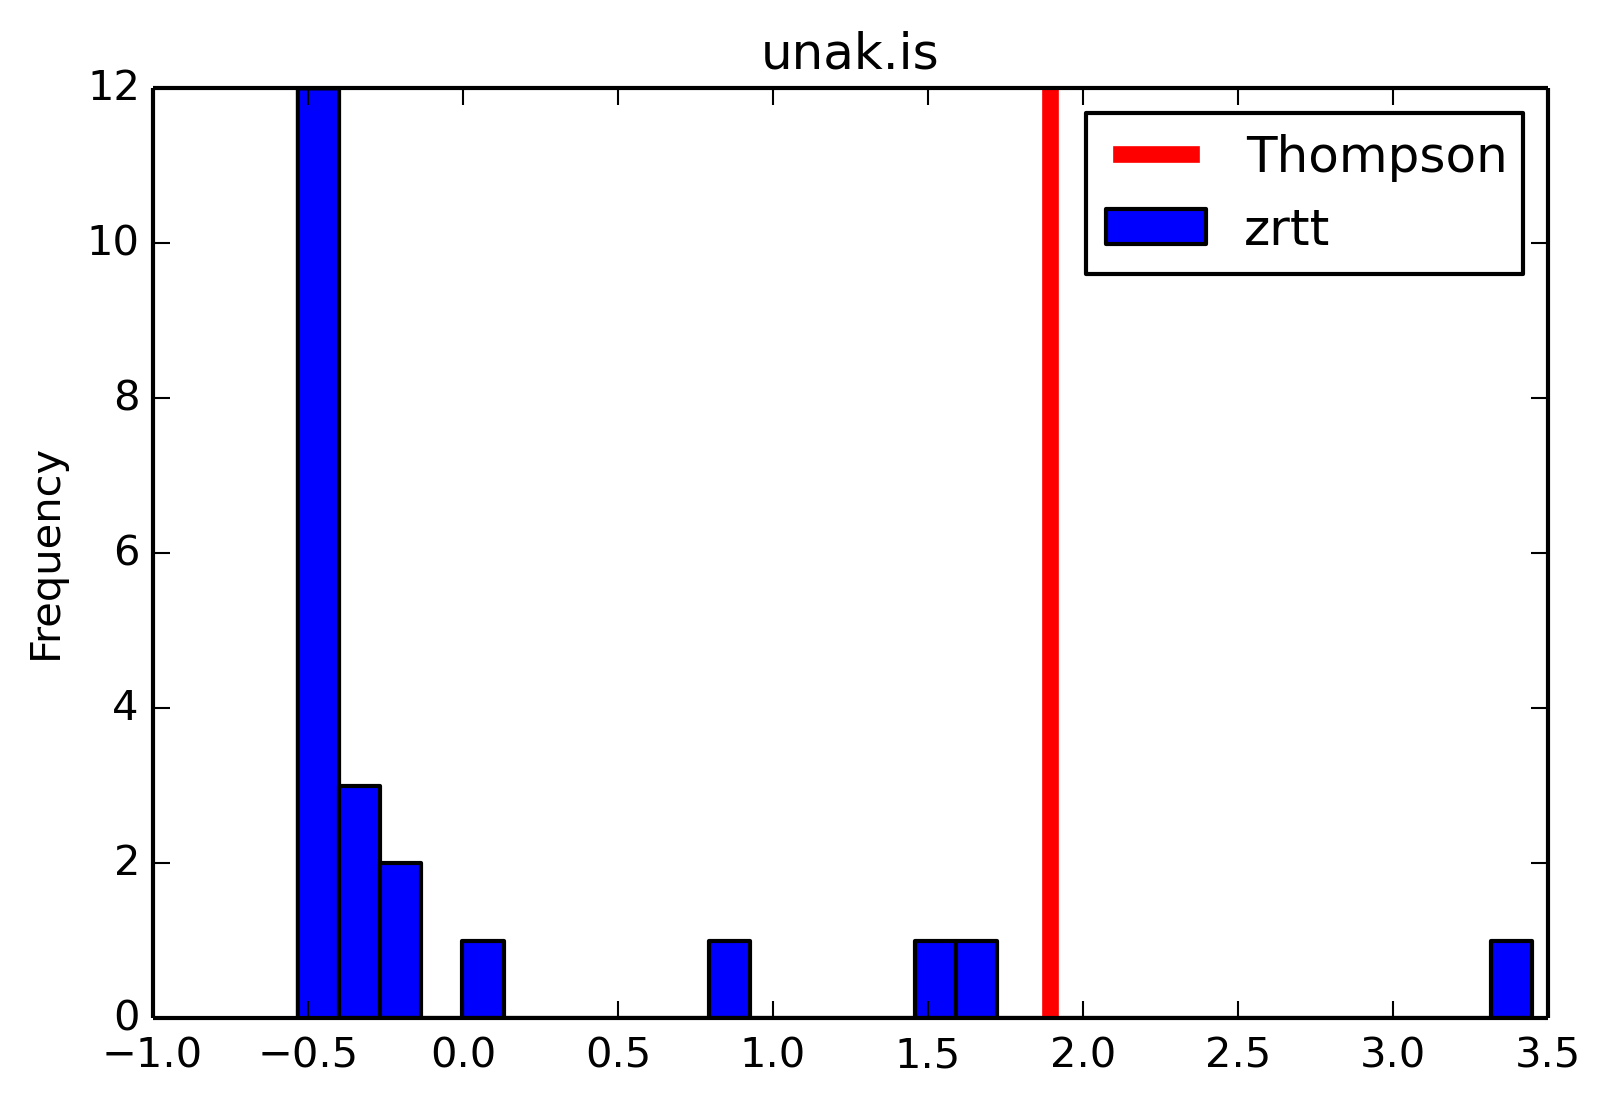
\includegraphics[width=0.45\textwidth]{histogramas_thompson/unak-is.png}
  \caption{RTT }
  \label{entropia-s}
\end{figure}

\begin{figure}[H]
  \centering
    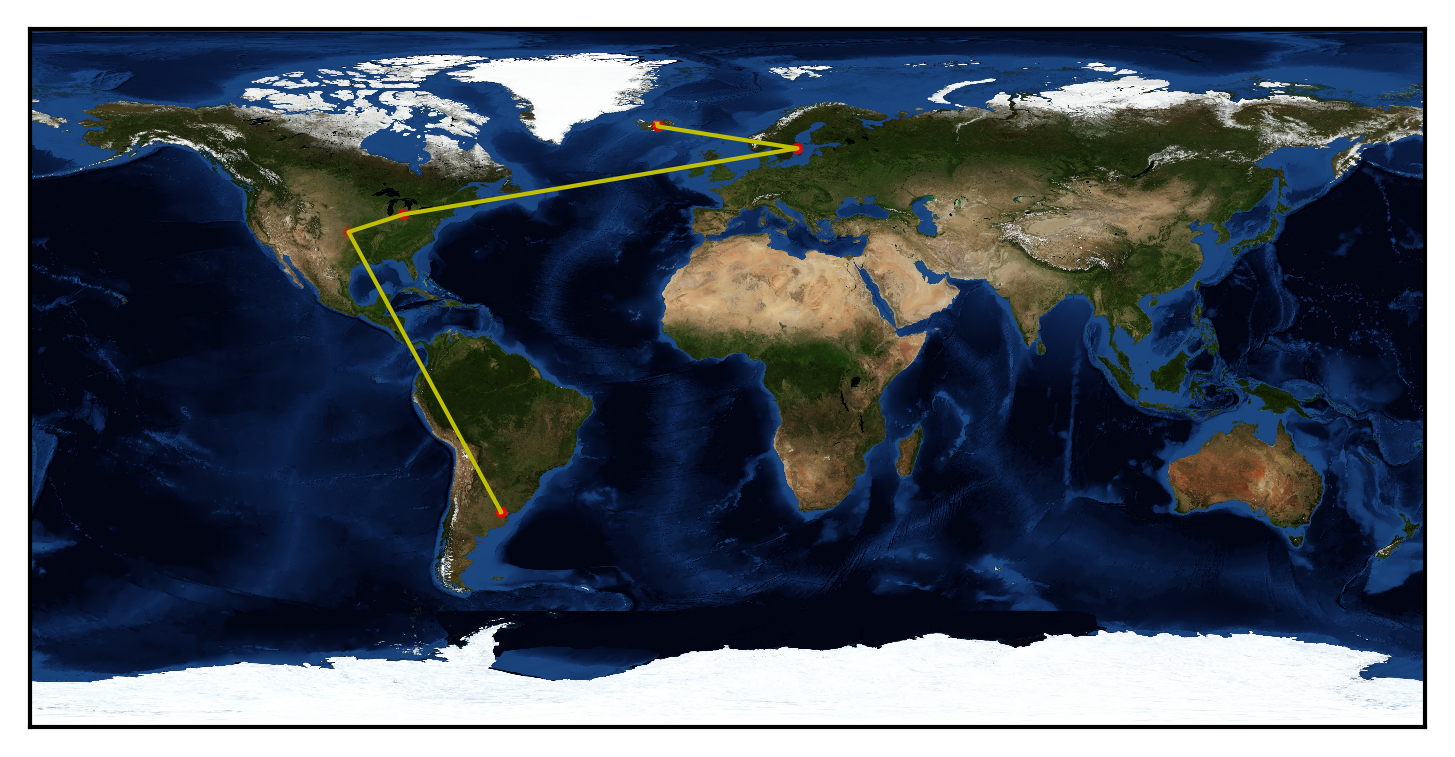
\includegraphics[width=0.45\textwidth]{grafico-rutas/unak-is.png}
  \caption{Gráfico de la ruta}
  \label{entropia-s}
\end{figure}




\subsection{Servidor unak.is}
\begin{figure}[H]
  \centering
    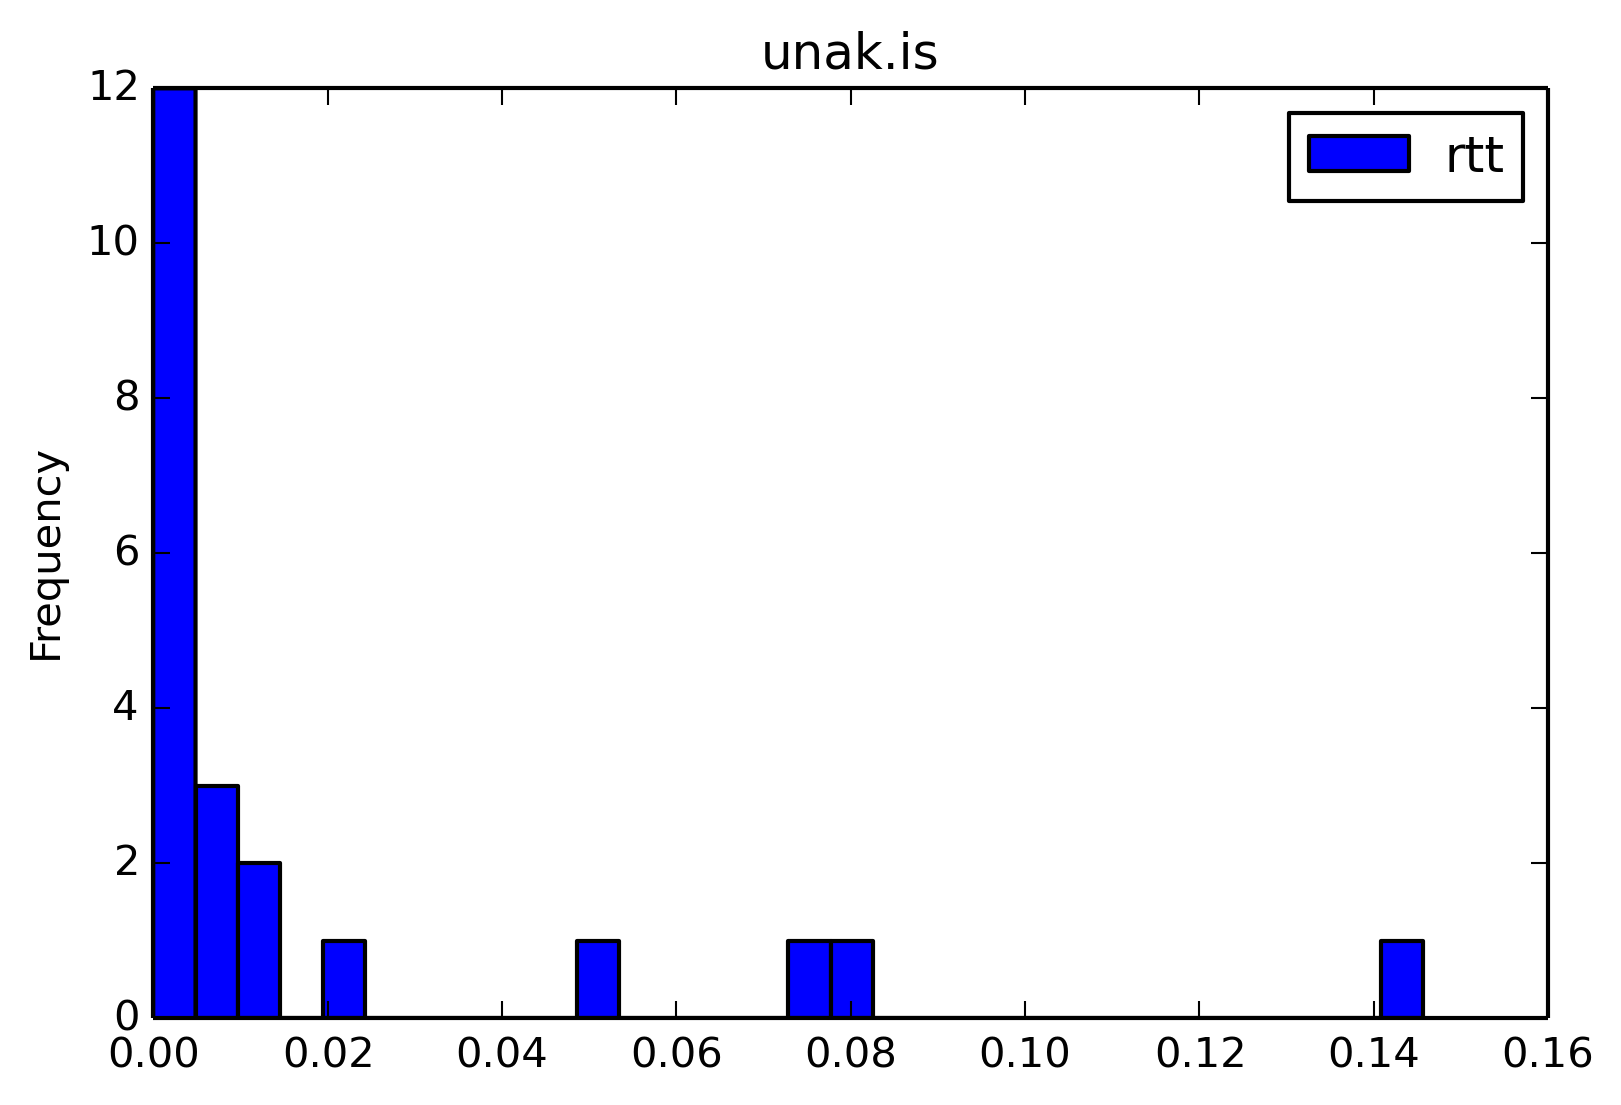
\includegraphics[width=0.45\textwidth]{histogramas_rtt/unak-is.png}
  \caption{RTT entre saltos}
  \label{entropia-s}
\end{figure}

\begin{figure}[H]
  \centering
    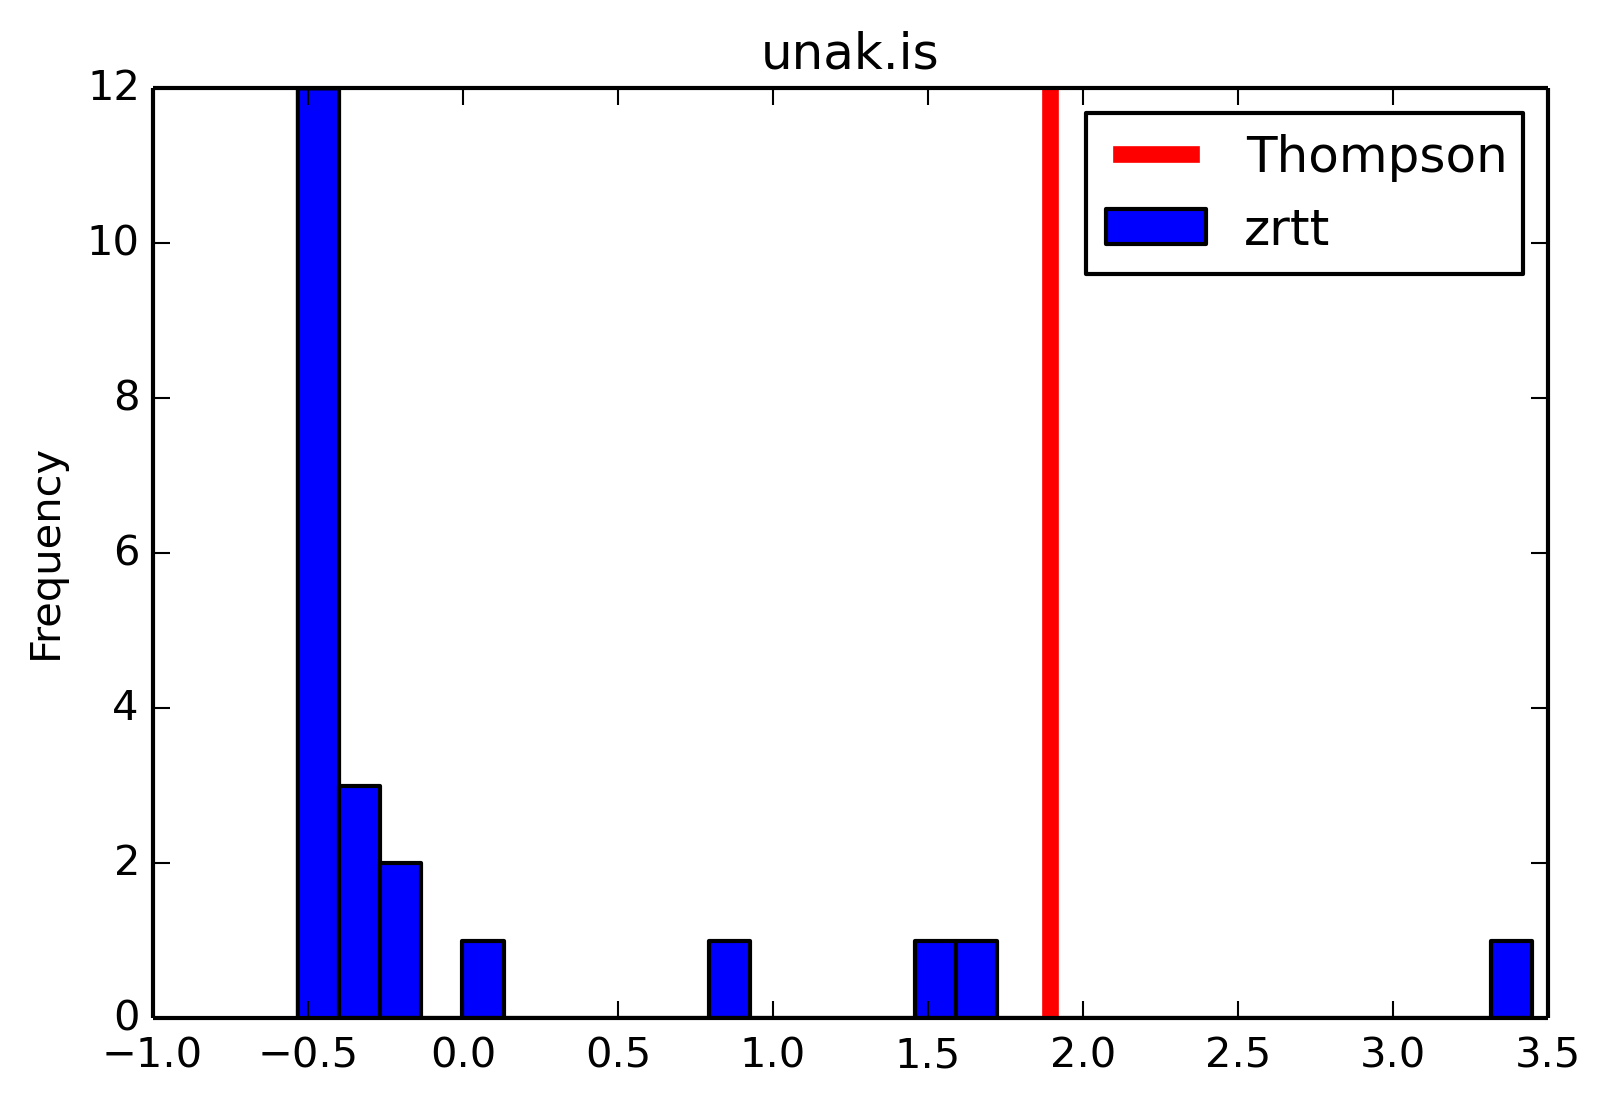
\includegraphics[width=0.45\textwidth]{histogramas_thompson/unak-is.png}
  \caption{RTT }
  \label{entropia-s}
\end{figure}

\begin{figure}[H]
  \centering
    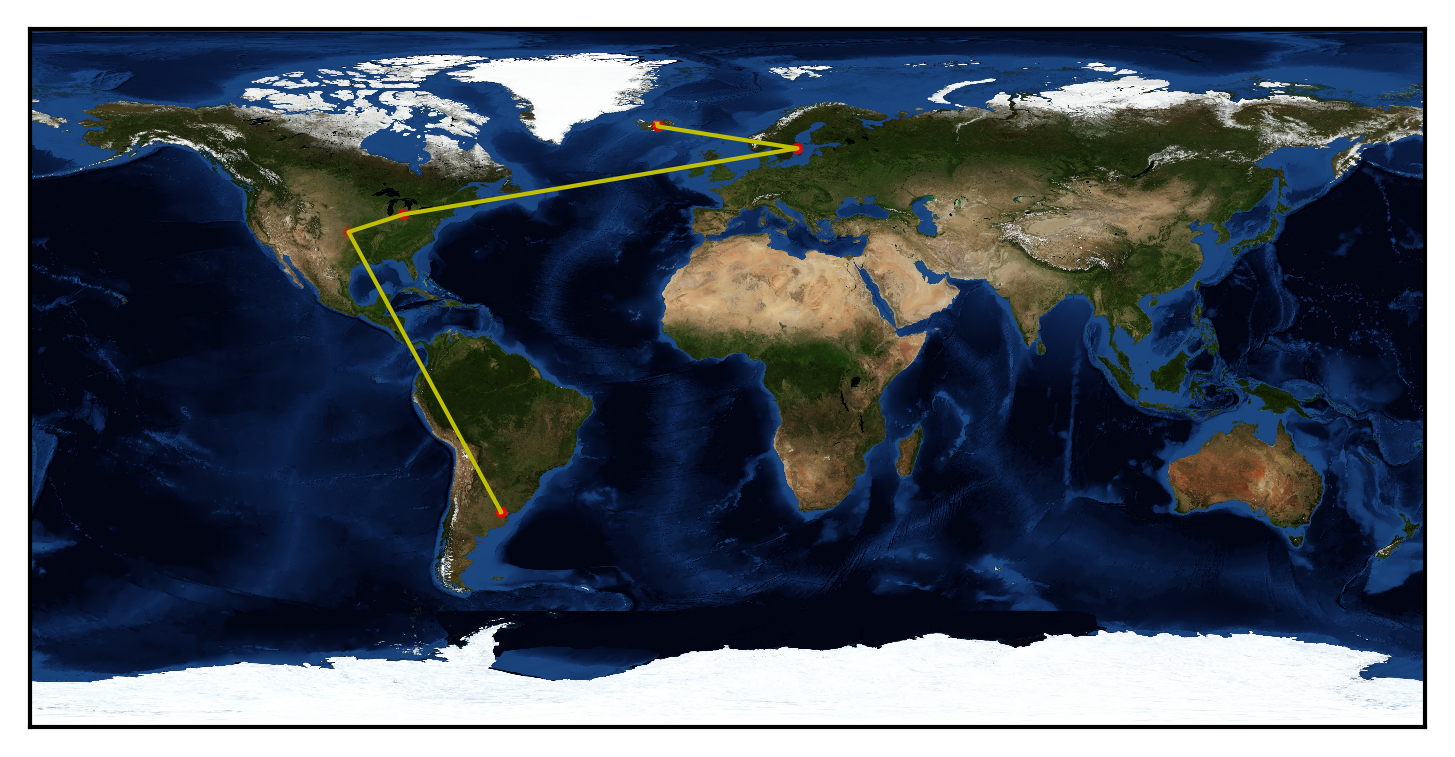
\includegraphics[width=0.45\textwidth]{grafico-rutas/unak-is.png}
  \caption{Gráfico de la ruta}
  \label{entropia-s}
\end{figure}




\subsection{Servidor unis.no}
\begin{figure}[H]
  \centering
    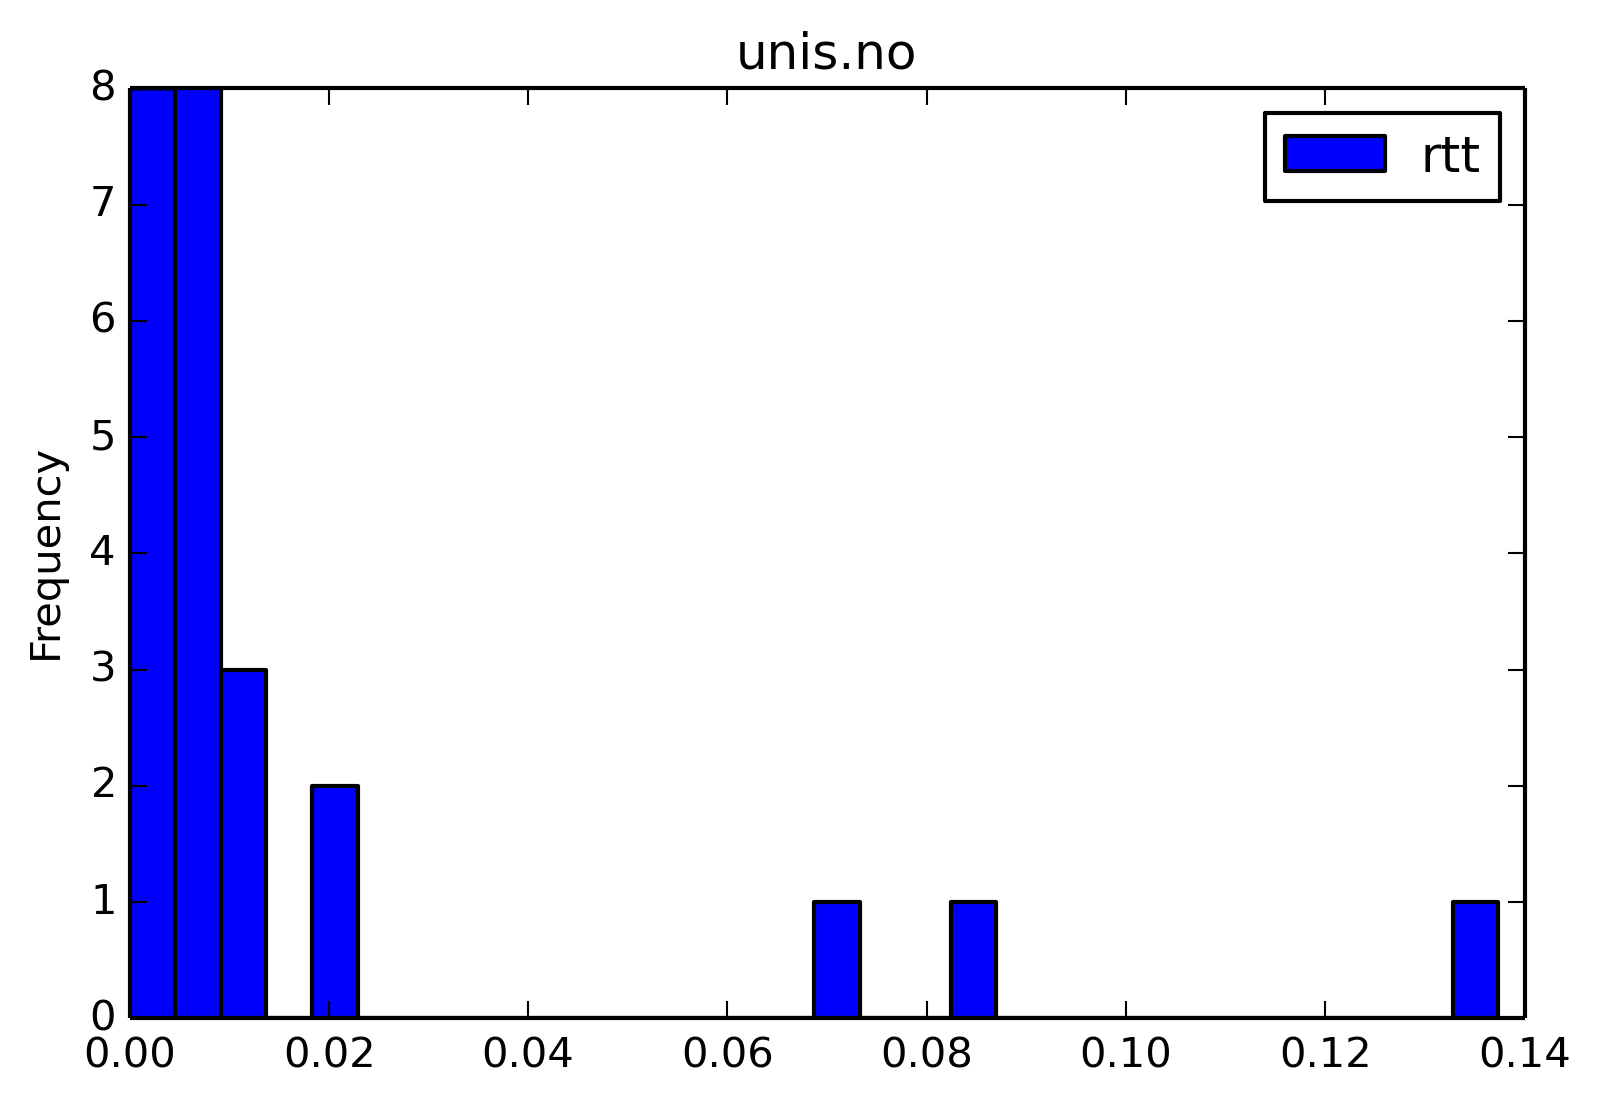
\includegraphics[width=0.45\textwidth]{histogramas_rtt/unis-no.png}
  \caption{RTT entre saltos}
  \label{entropia-s}
\end{figure}

\begin{figure}[H]
  \centering
    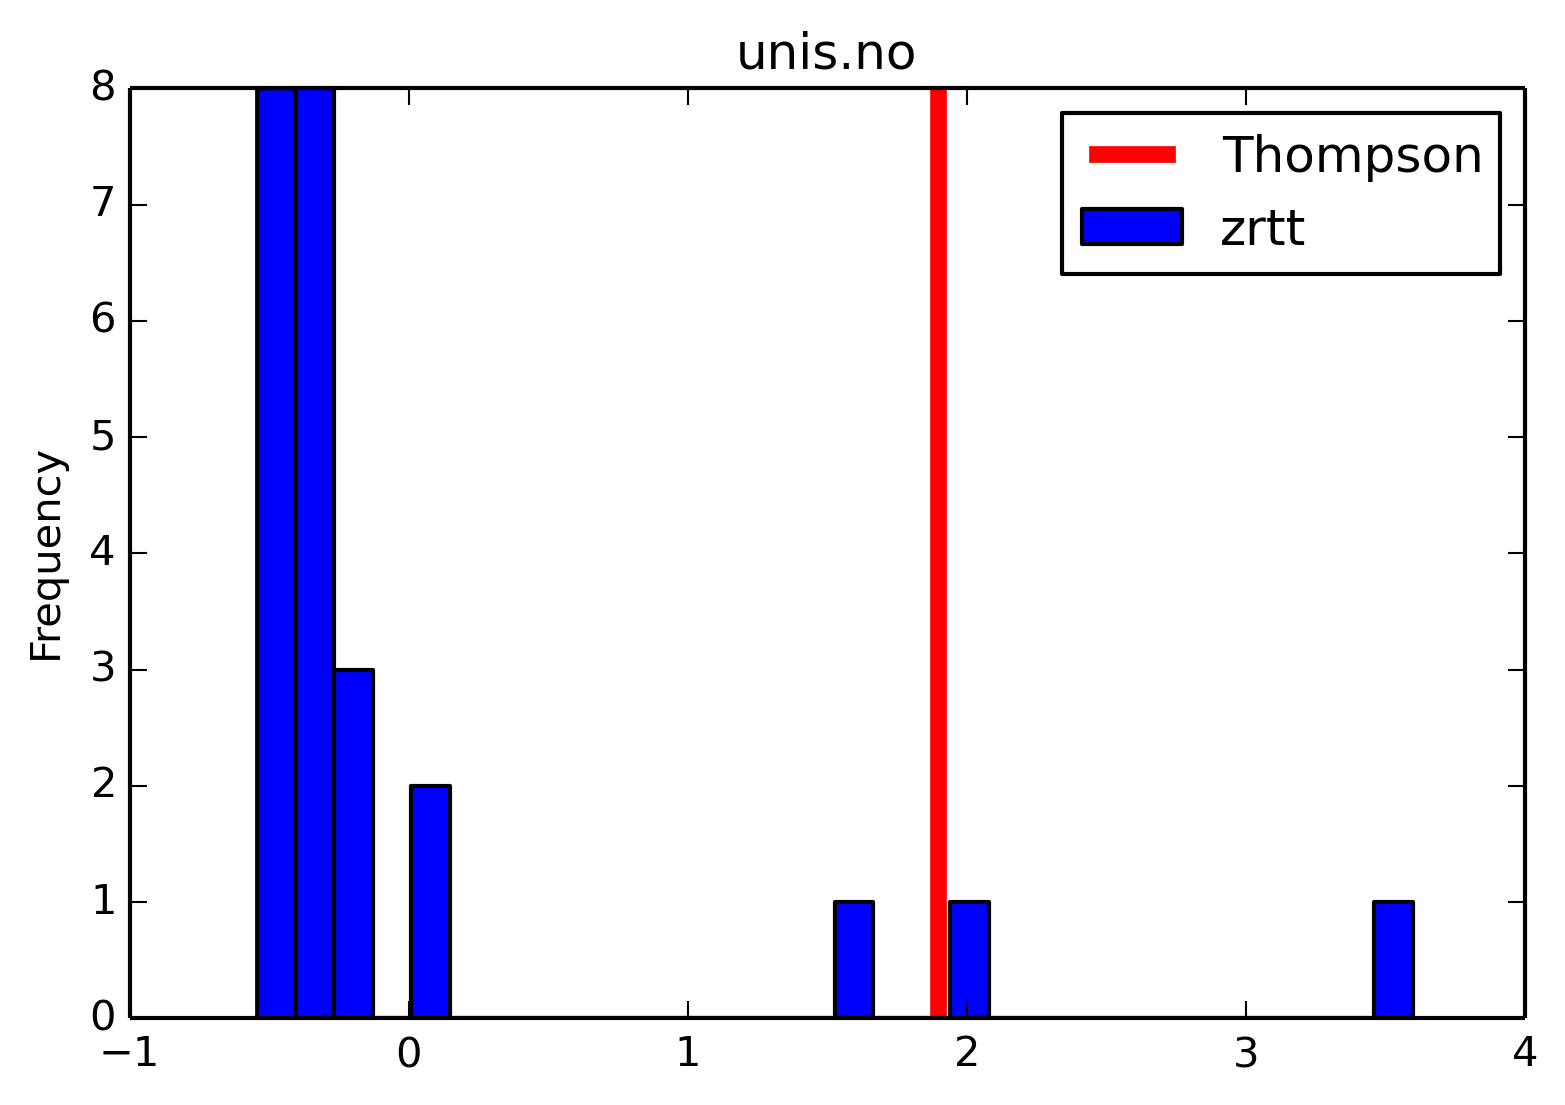
\includegraphics[width=0.45\textwidth]{histogramas_thompson/unis-no.png}
  \caption{RTTs Normailzados comparados con el valor Thompson}
  \label{entropia-s}
\end{figure}

\begin{figure}[H]
  \centering
    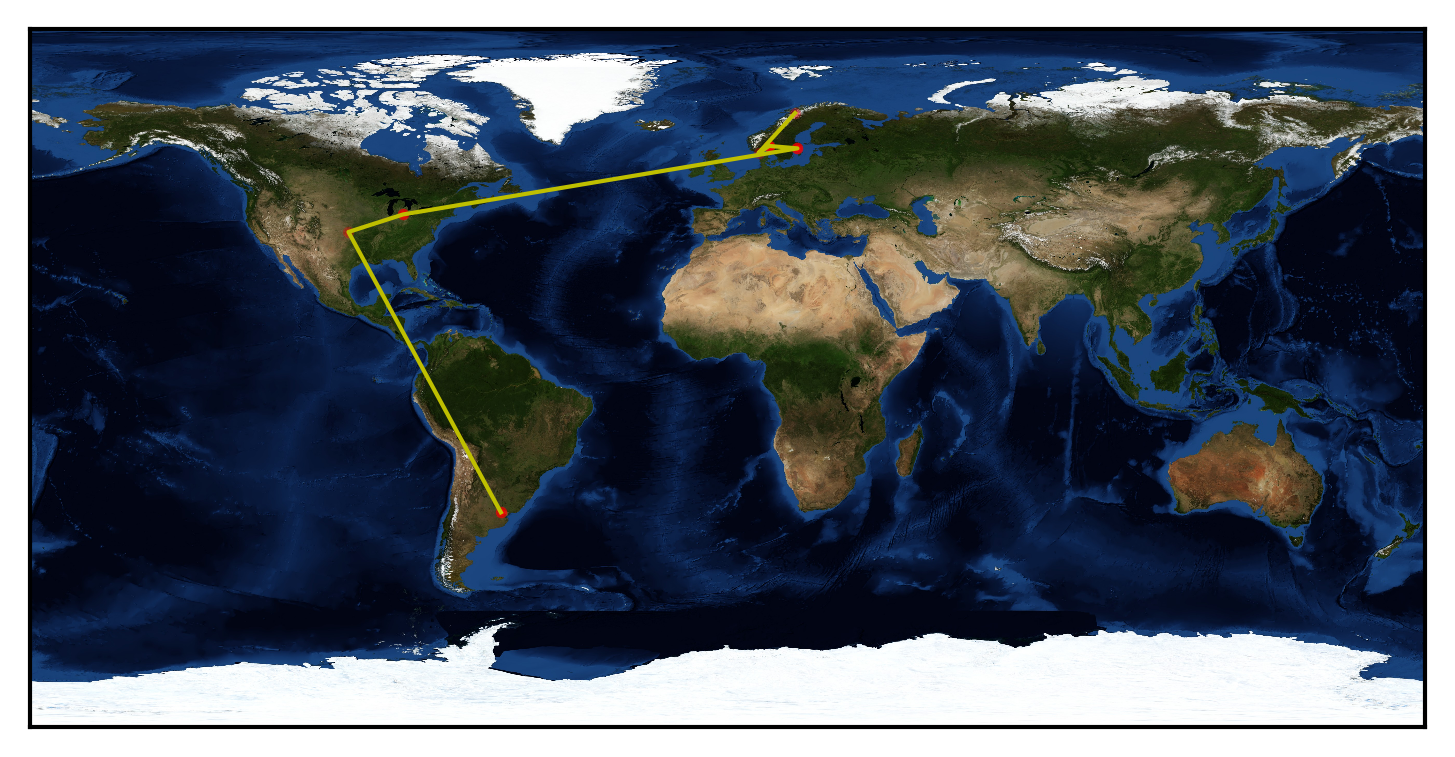
\includegraphics[width=0.45\textwidth]{grafico-rutas/unis-no.png}
  \caption{Gráfico de la ruta}
  \label{entropia-s}
\end{figure}




\subsection{Servidor www.fu-berlin.de}
\begin{figure}[H]
  \centering
    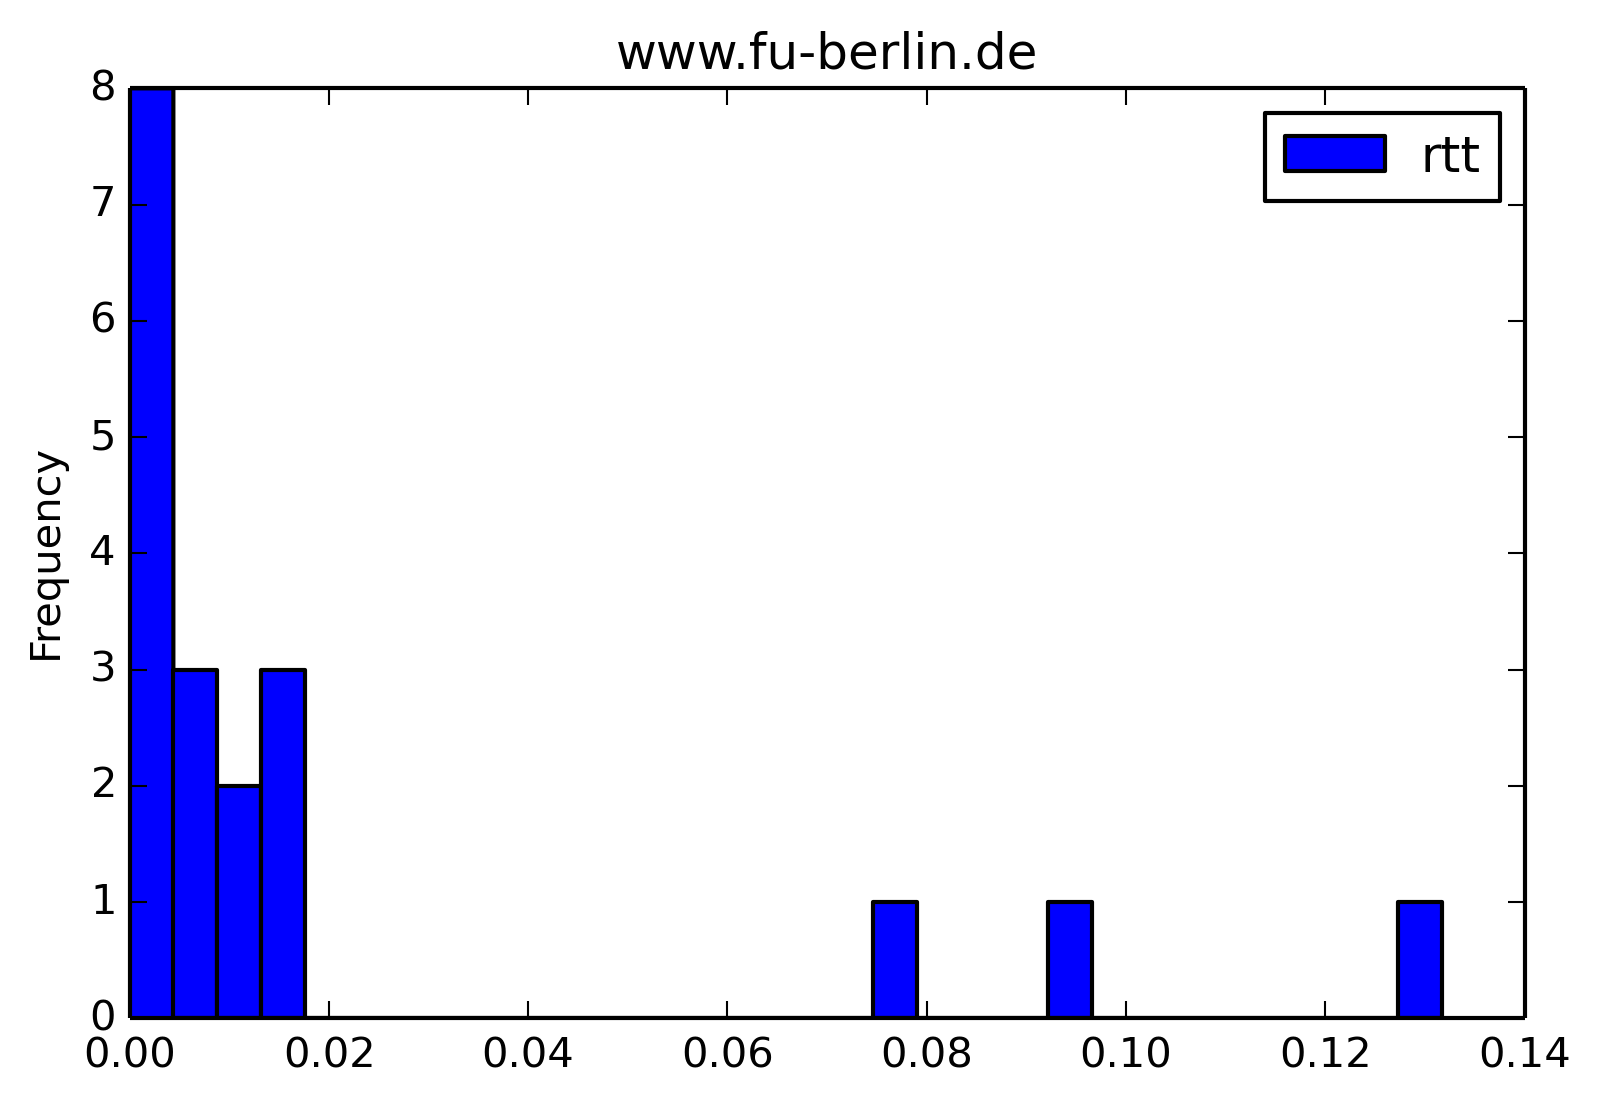
\includegraphics[width=0.45\textwidth]{histogramas_rtt/www-fu-berlin-de.png}
  \caption{RTT entre saltos}
  \label{entropia-s}
\end{figure}

\begin{figure}[H]
  \centering
    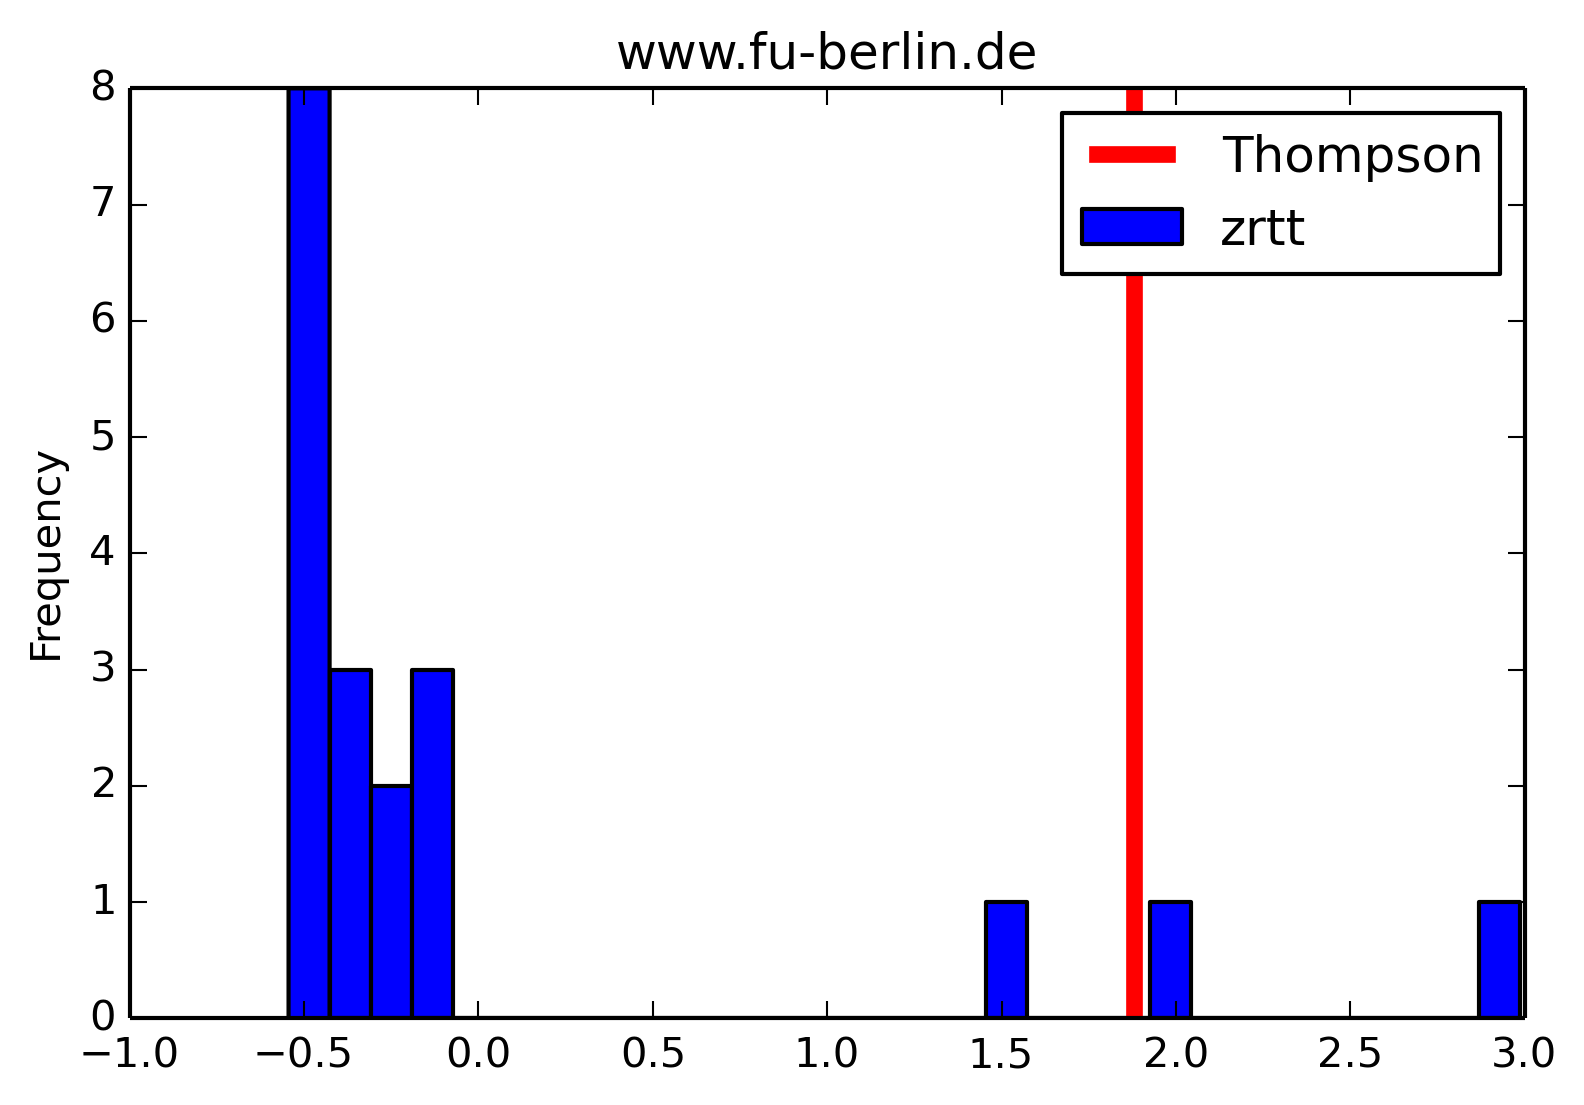
\includegraphics[width=0.45\textwidth]{histogramas_thompson/www-fu-berlin-de.png}
  \caption{RTTs Normailzados comparados con el valor Thompson}
  \label{entropia-s}
\end{figure}

\begin{figure}[H]
  \centering
    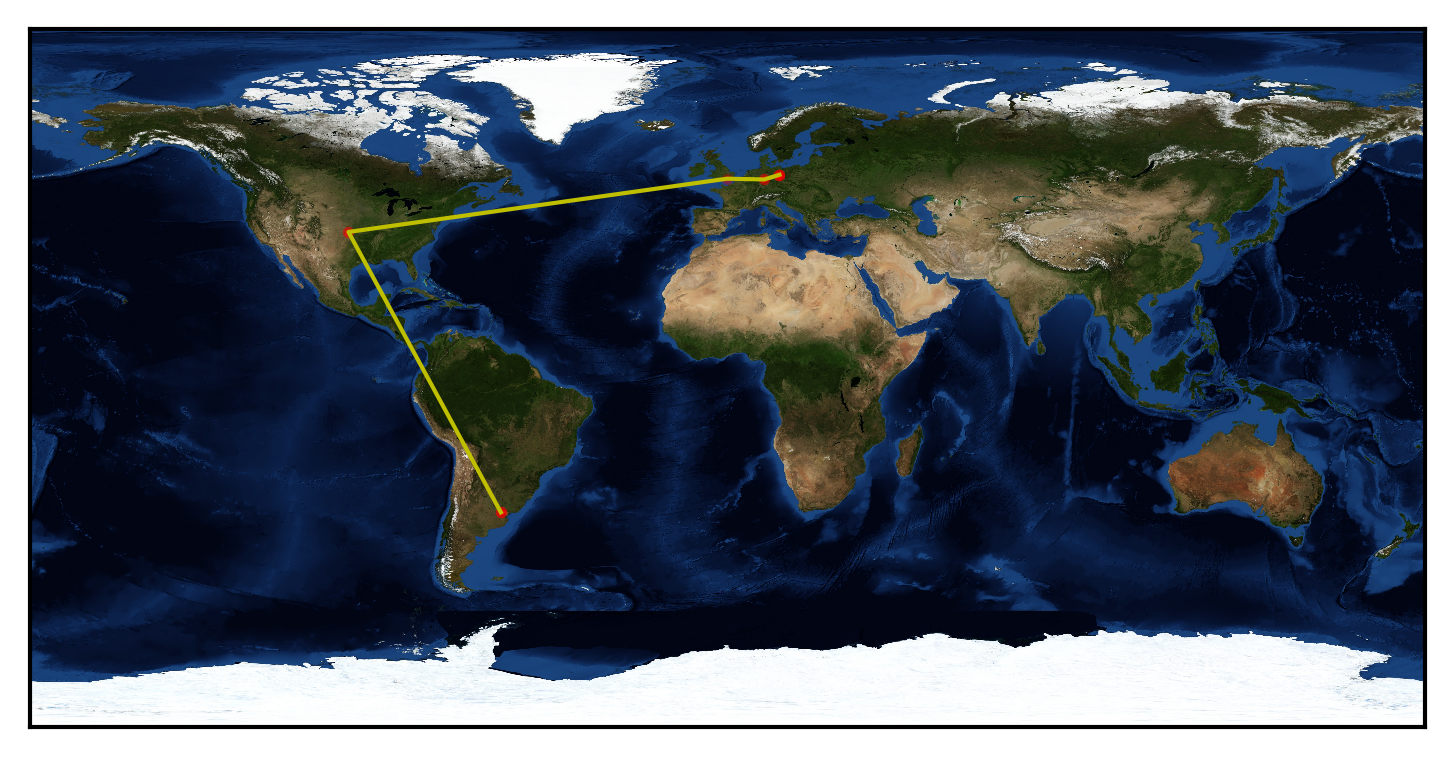
\includegraphics[width=0.45\textwidth]{grafico-rutas/www-fu-berlin-de.png}
  \caption{Gráfico de la ruta}
  \label{entropia-s}
\end{figure}




\subsection{Servidor www.kstu.kz}
\begin{figure}[H]
  \centering
    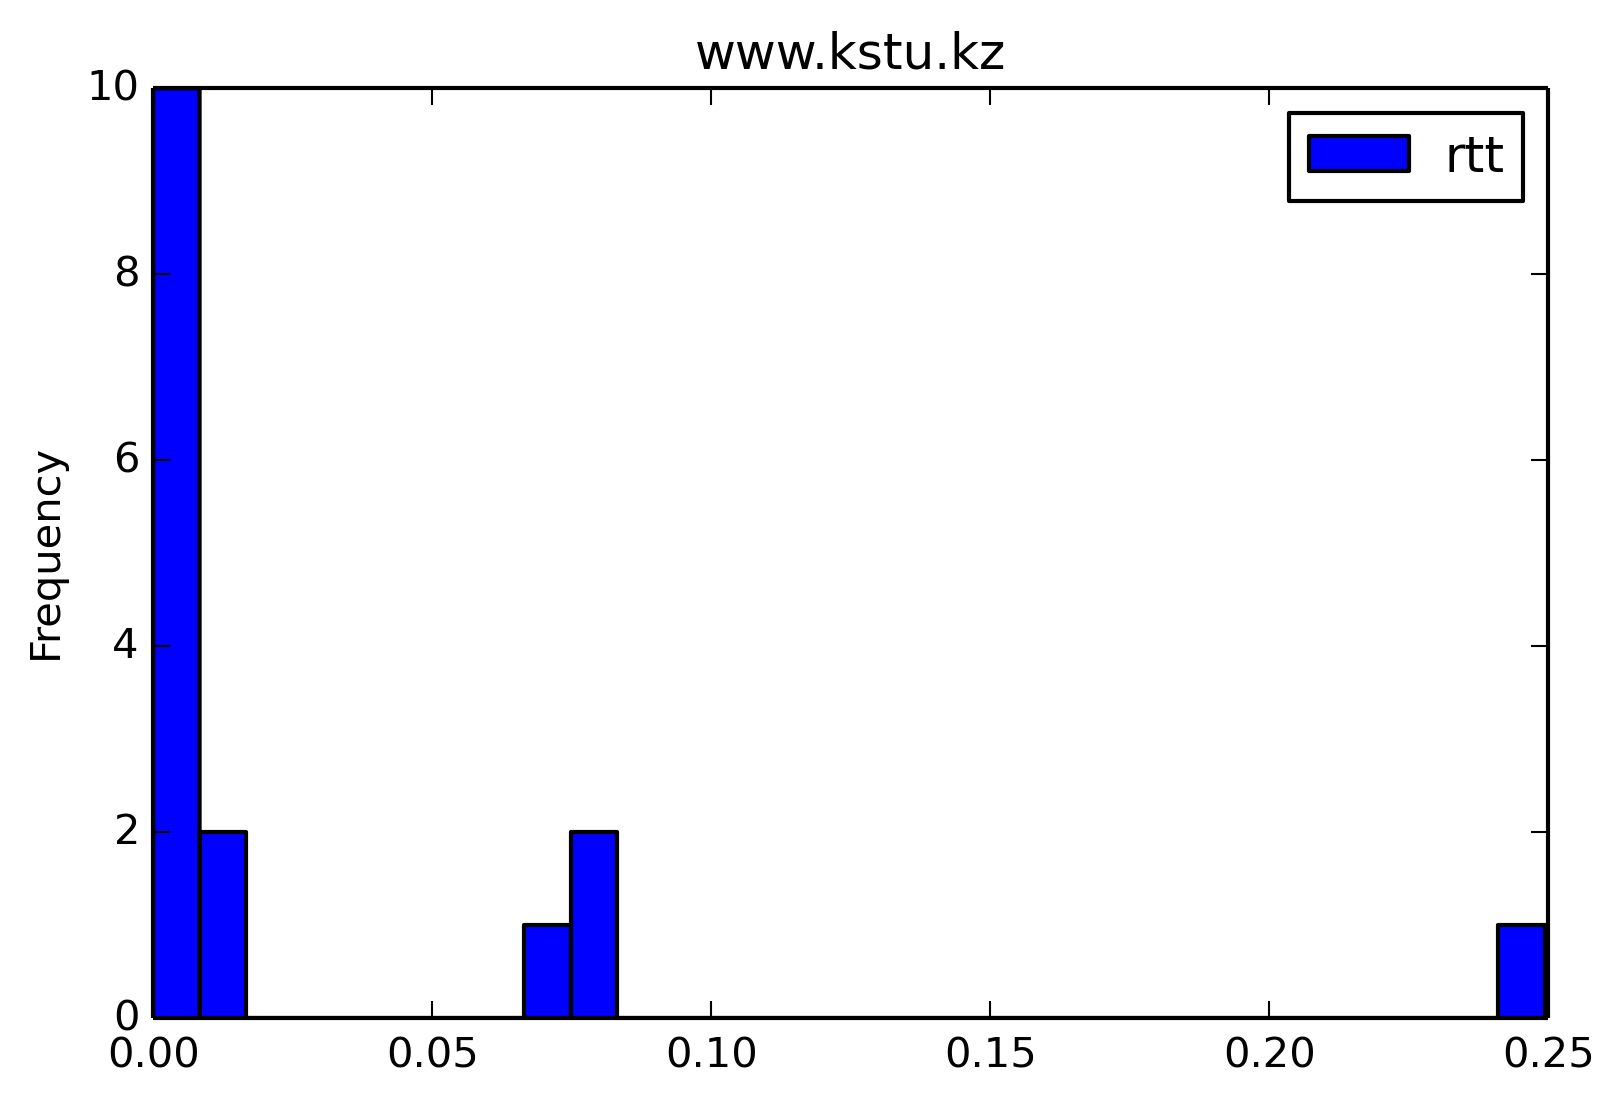
\includegraphics[width=0.45\textwidth]{histogramas_rtt/www-kstu-kz.png}
  \caption{RTT entre saltos}
  \label{entropia-s}
\end{figure}

\begin{figure}[H]
  \centering
    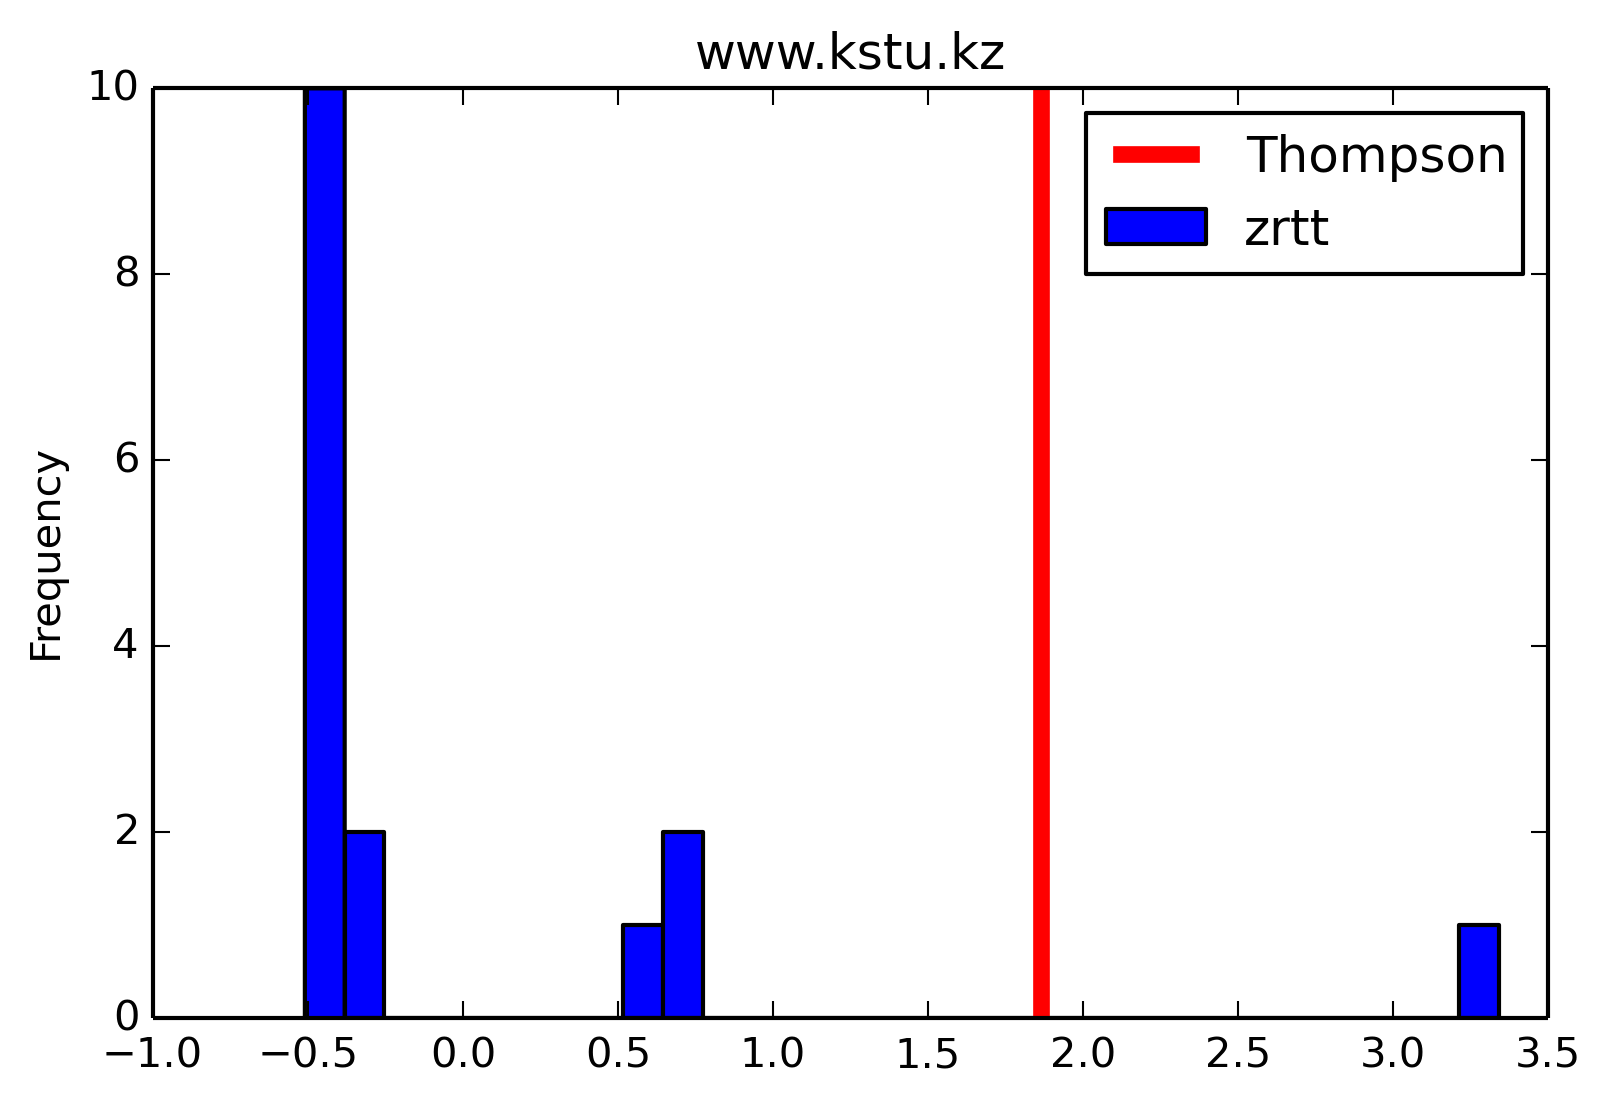
\includegraphics[width=0.45\textwidth]{histogramas_thompson/www-kstu-kz.png}
  \caption{RTTs Normailzados comparados con el valor Thompson}
  \label{entropia-s}
\end{figure}

\begin{figure}[H]
  \centering
    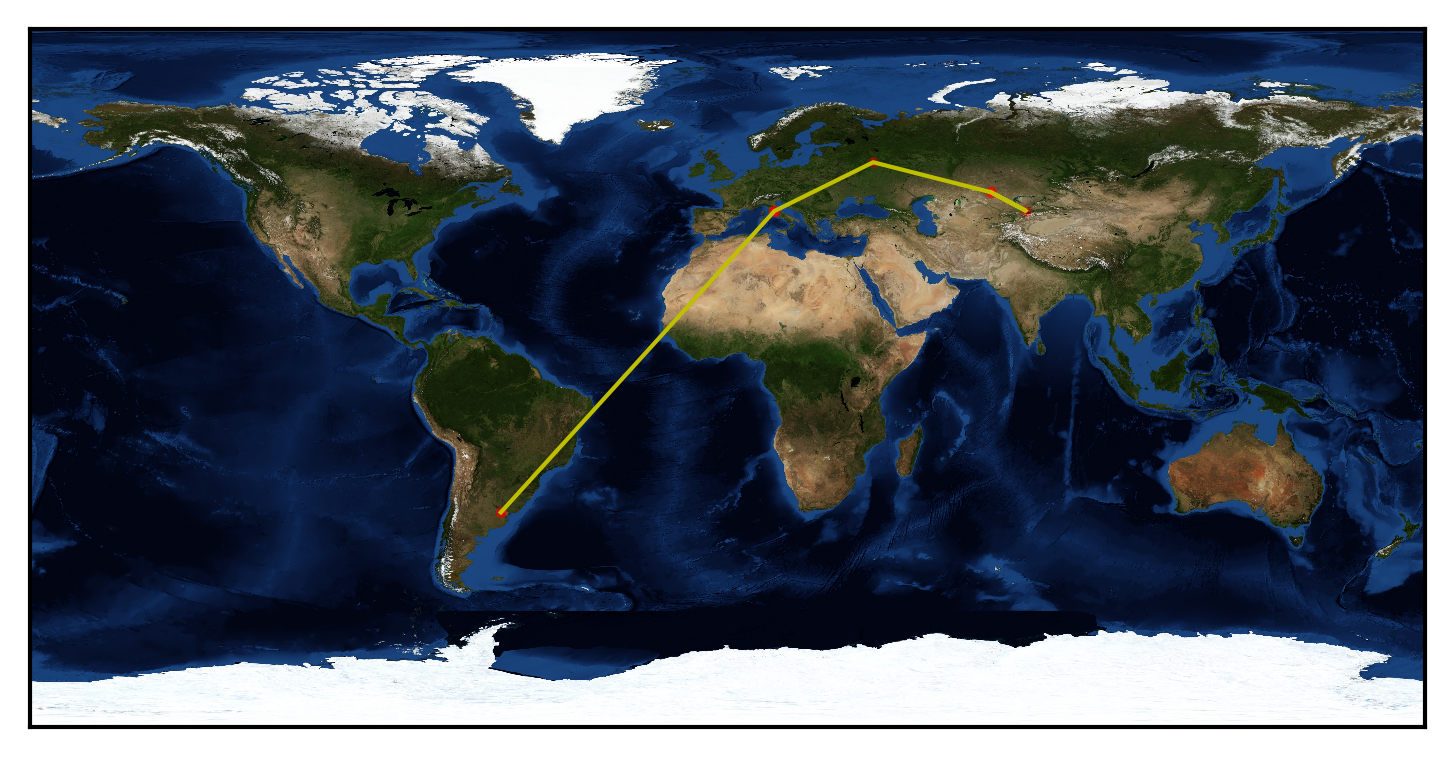
\includegraphics[width=0.45\textwidth]{grafico-rutas/www-kstu-kz.png}
  \caption{Gráfico de la ruta}
  \label{entropia-s}
\end{figure}




\subsection{Servidor www.uq.edu.au}
\begin{figure}[H]
  \centering
    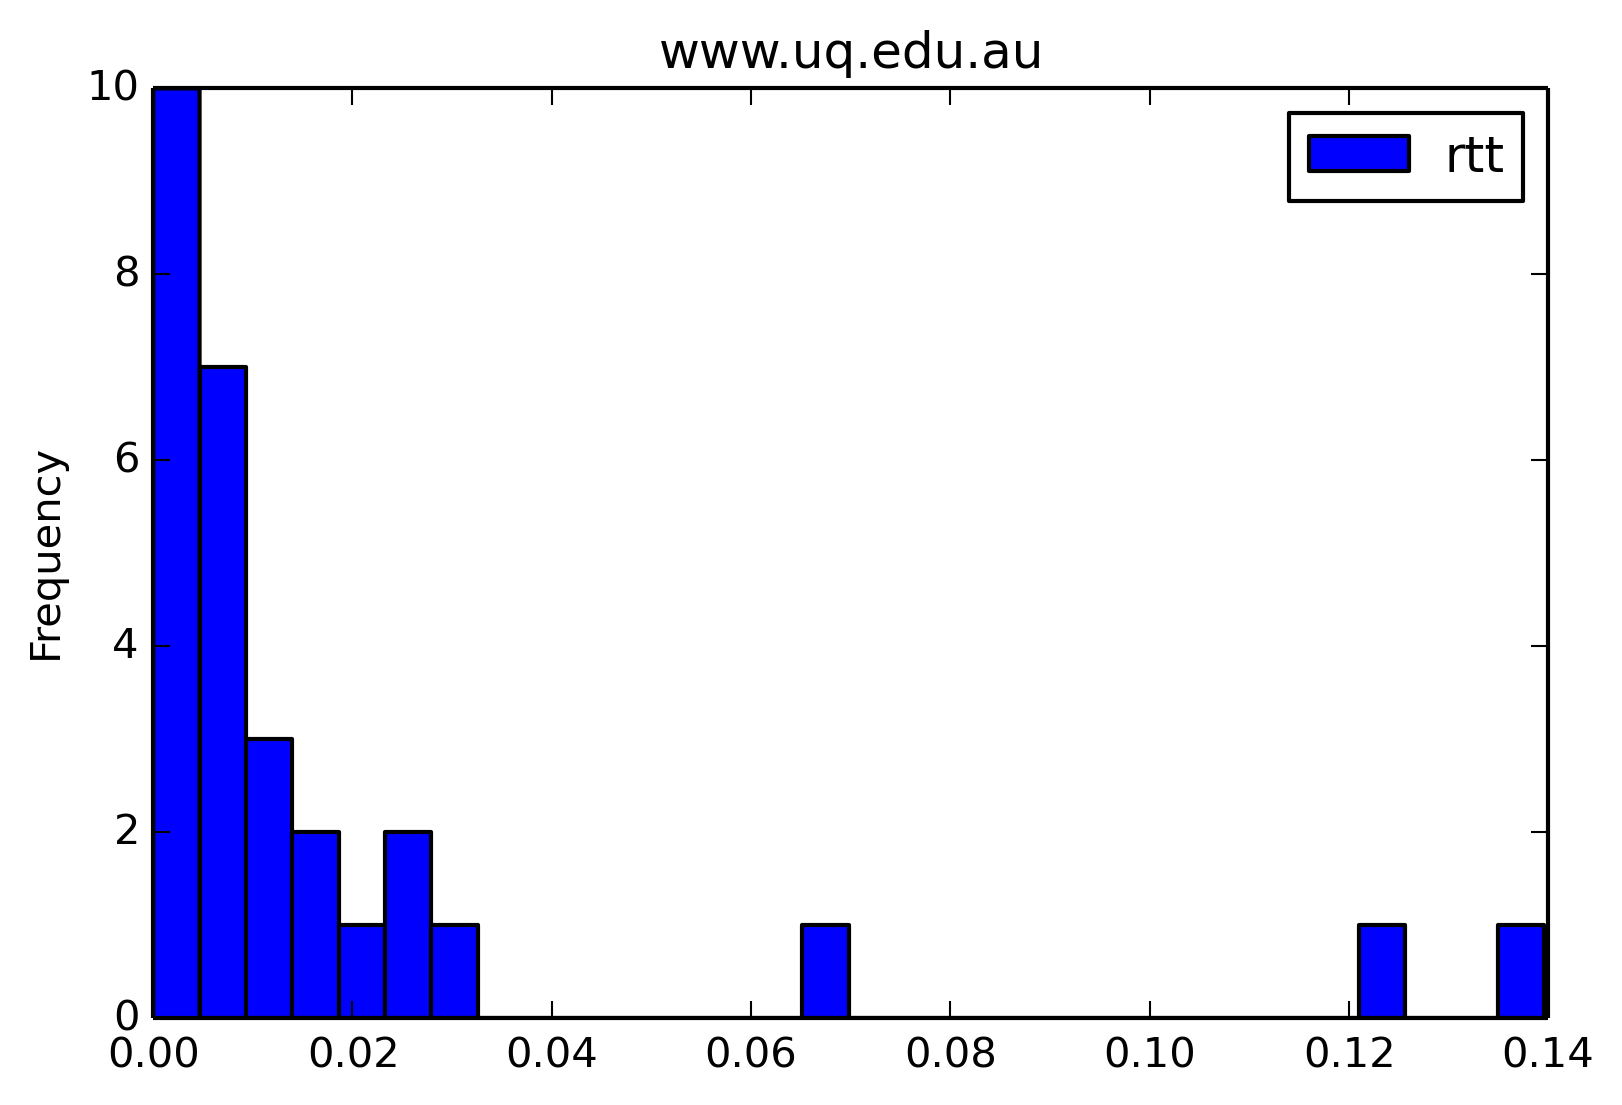
\includegraphics[width=0.45\textwidth]{histogramas_rtt/www-uq-edu-au.png}
  \caption{RTT entre saltos}
  \label{entropia-s}
\end{figure}

\begin{figure}[H]
  \centering
    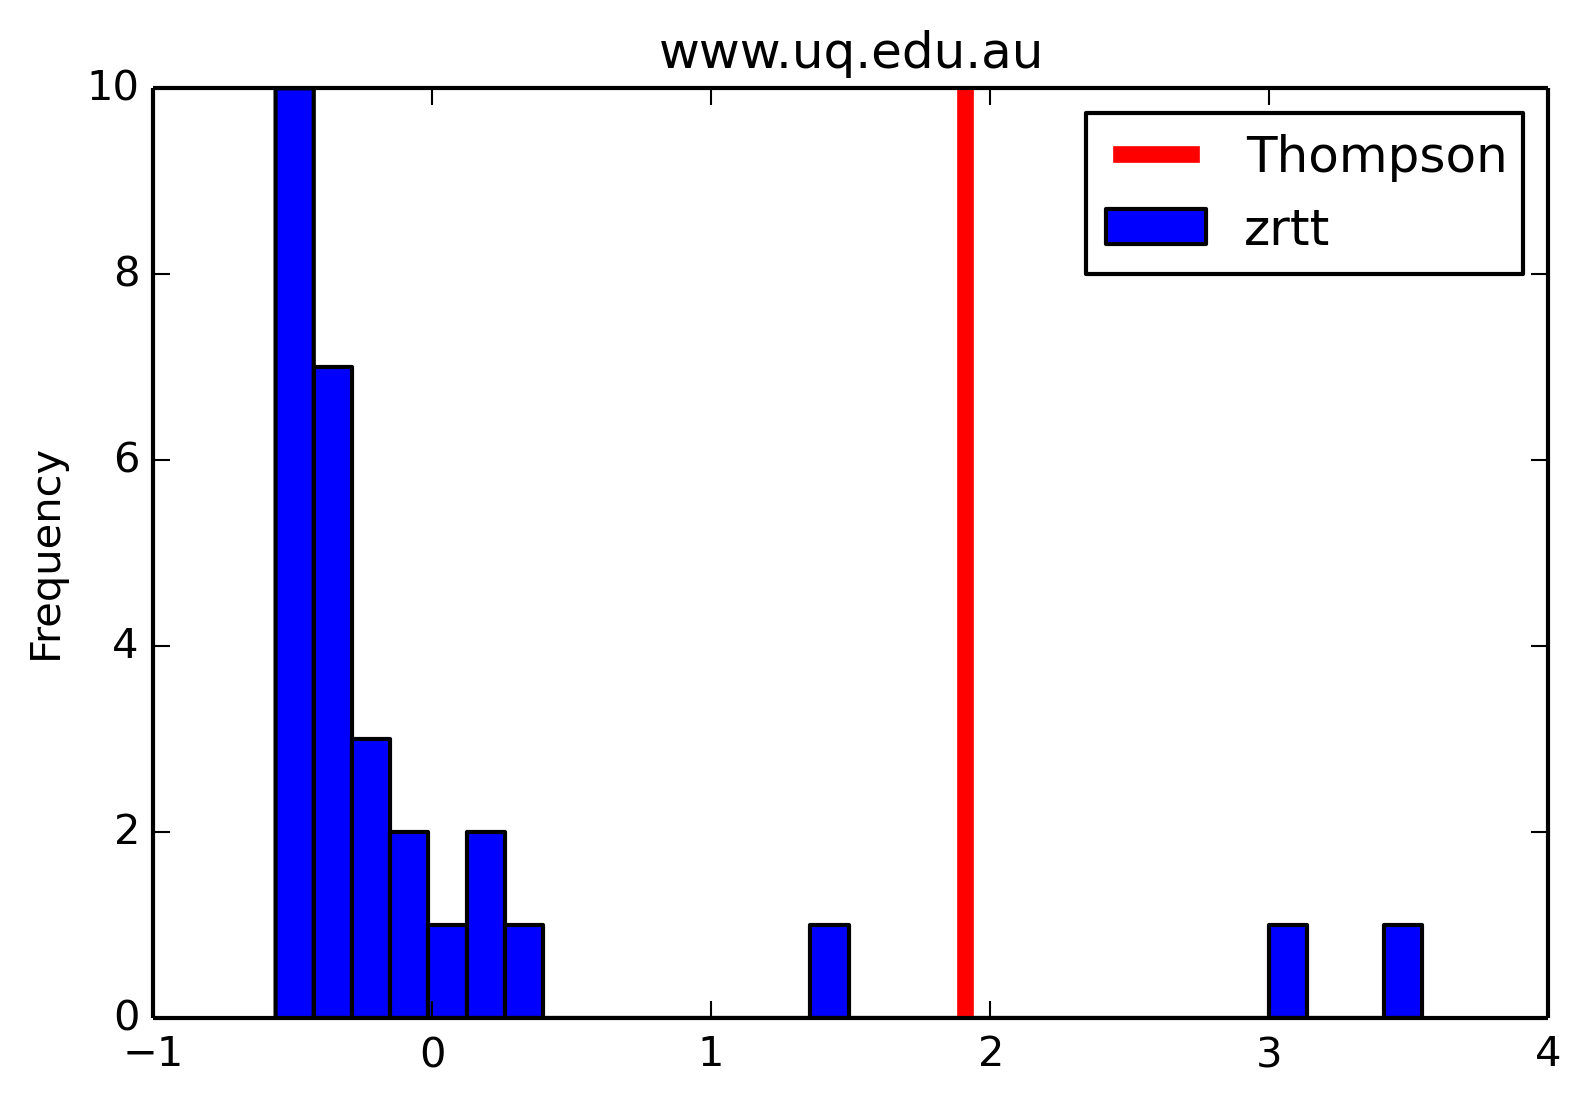
\includegraphics[width=0.45\textwidth]{histogramas_thompson/www-uq-edu-au.png}
  \caption{RTTs Normailzados comparados con el valor Thompson}
  \label{entropia-s}
\end{figure}

\begin{figure}[H]
  \centering
    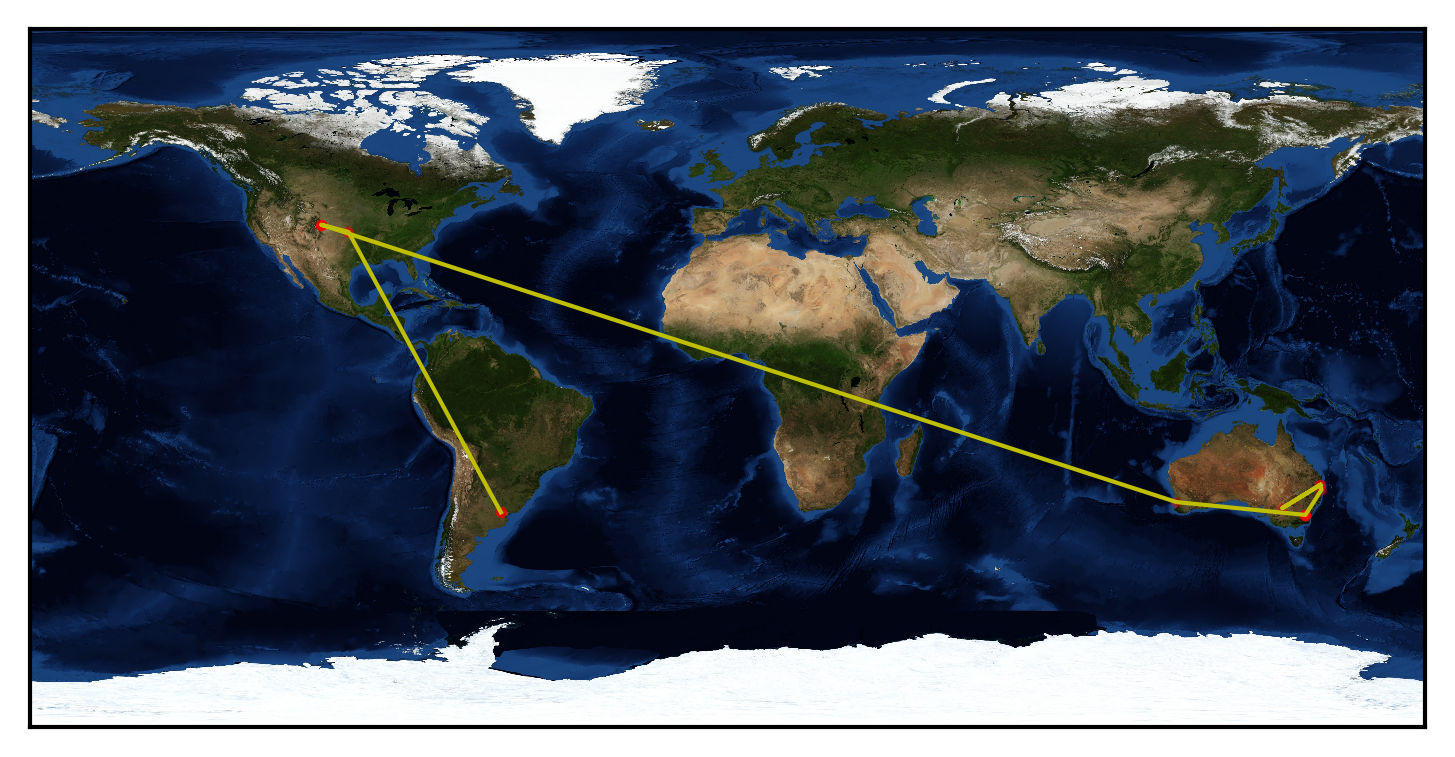
\includegraphics[width=0.45\textwidth]{grafico-rutas/www-uq-edu-au.png}
  \caption{Gráfico de la ruta}
  \label{entropia-s}
\end{figure}





\subsection{Servidor auckland.ac.nz}
\begin{figure}[H]
  \centering
    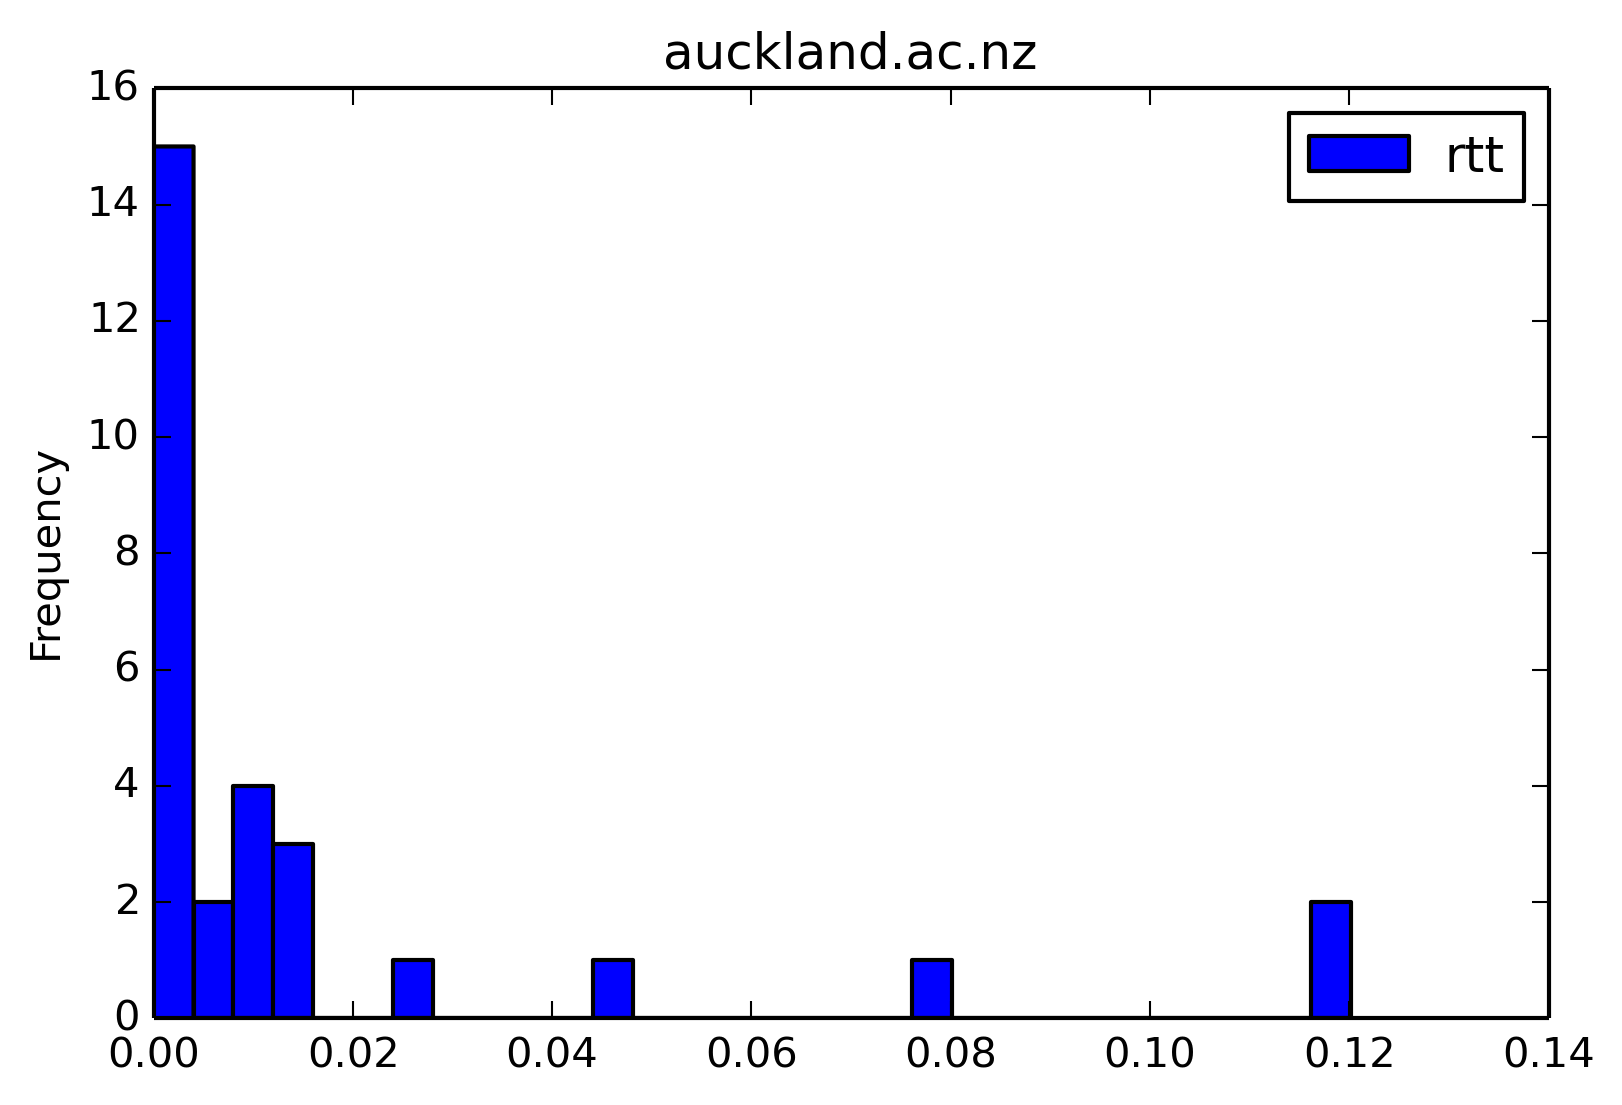
\includegraphics[width=0.45\textwidth]{histogramas_rtt/auckland-ac-nz.png}
  \caption{RTT entre saltos}
  \label{entropia-s}
\end{figure}

\begin{figure}[H]
  \centering
    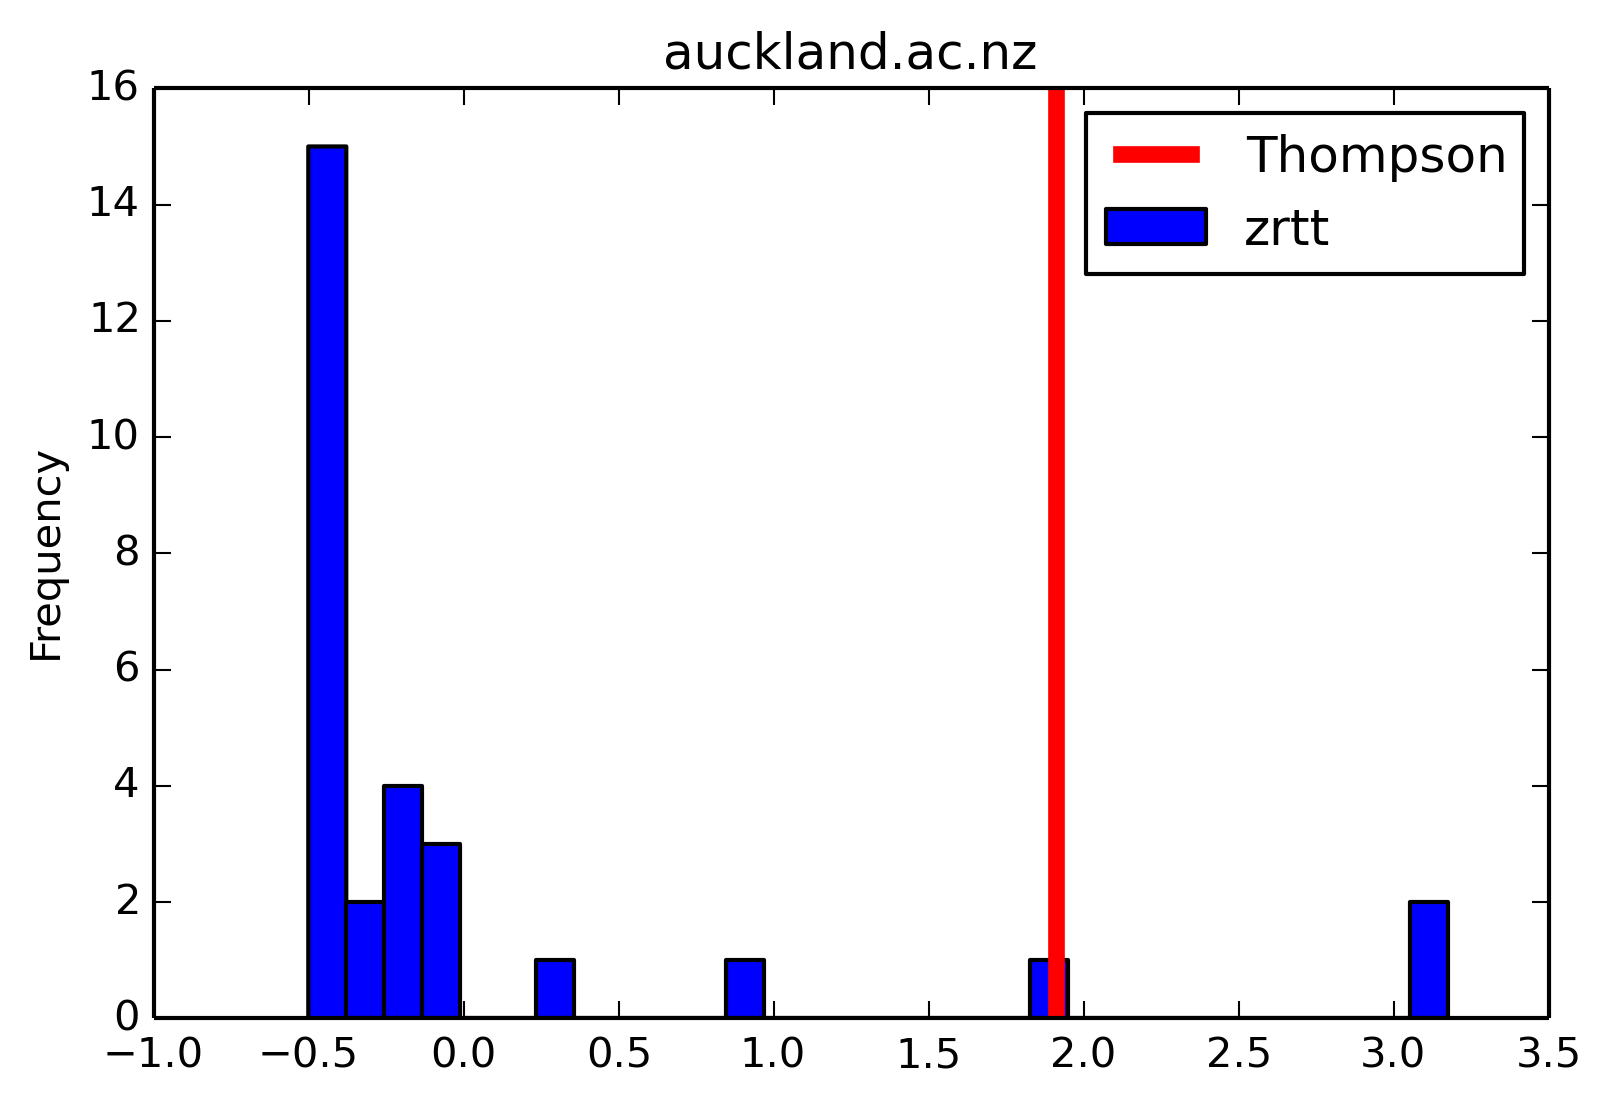
\includegraphics[width=0.45\textwidth]{histogramas_thompson/auckland-ac-nz.png}
  \caption{RTTs Normalizados comparados con el valor Thompson}
  \label{entropia-s}
\end{figure}

\begin{figure}[H]
  \centering
    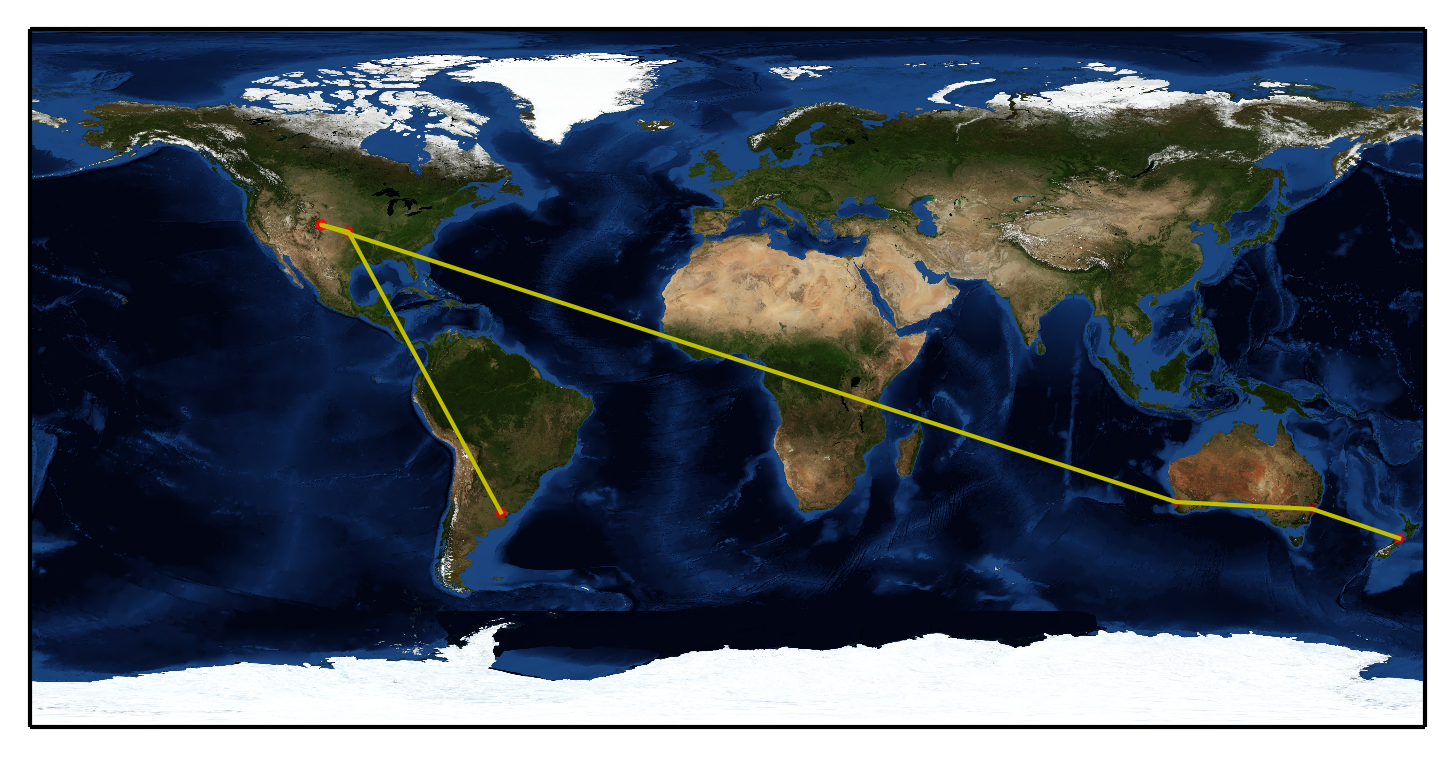
\includegraphics[width=0.45\textwidth]{grafico-rutas/auckland-ac-nz.png}
  \caption{Gráfico de la ruta}
  \label{entropia-s}
\end{figure}




\subsection{Servidor invertisuniversity.ac.in}
\begin{figure}[H]
  \centering
    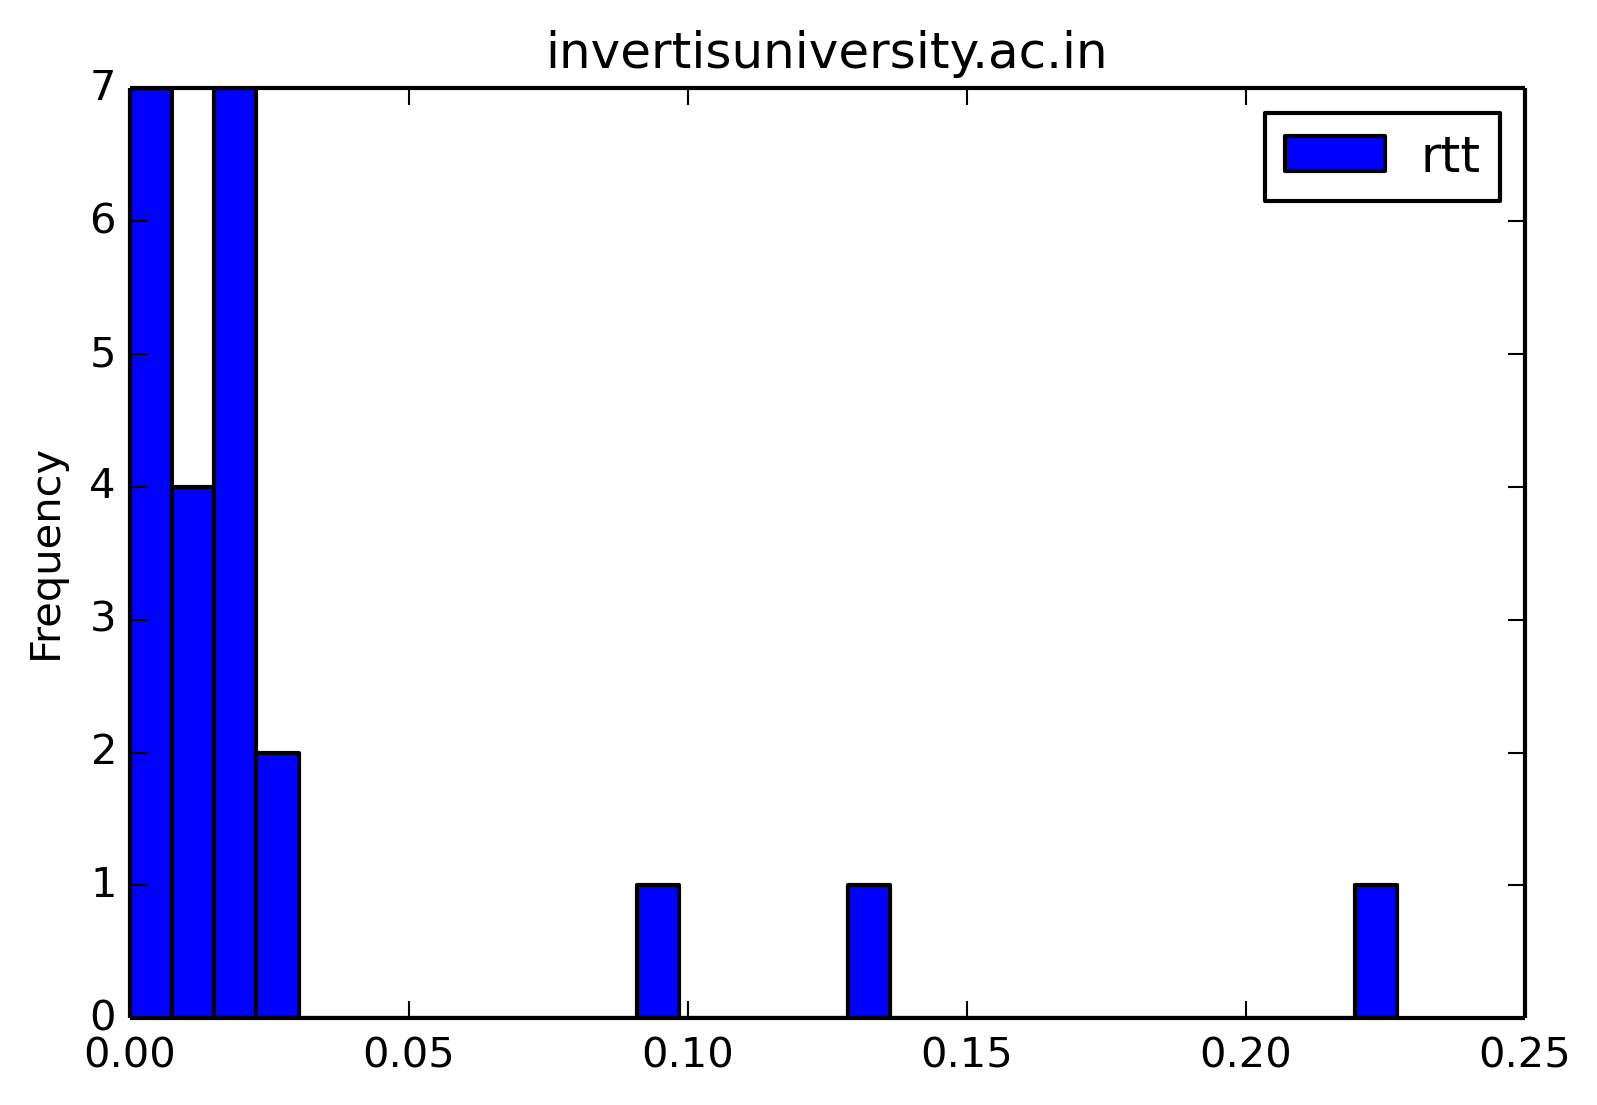
\includegraphics[width=0.45\textwidth]{histogramas_rtt/invertisuniversity-ac-in.png}
  \caption{RTT entre saltos}
  \label{entropia-s}
\end{figure}

\begin{figure}[H]
  \centering
    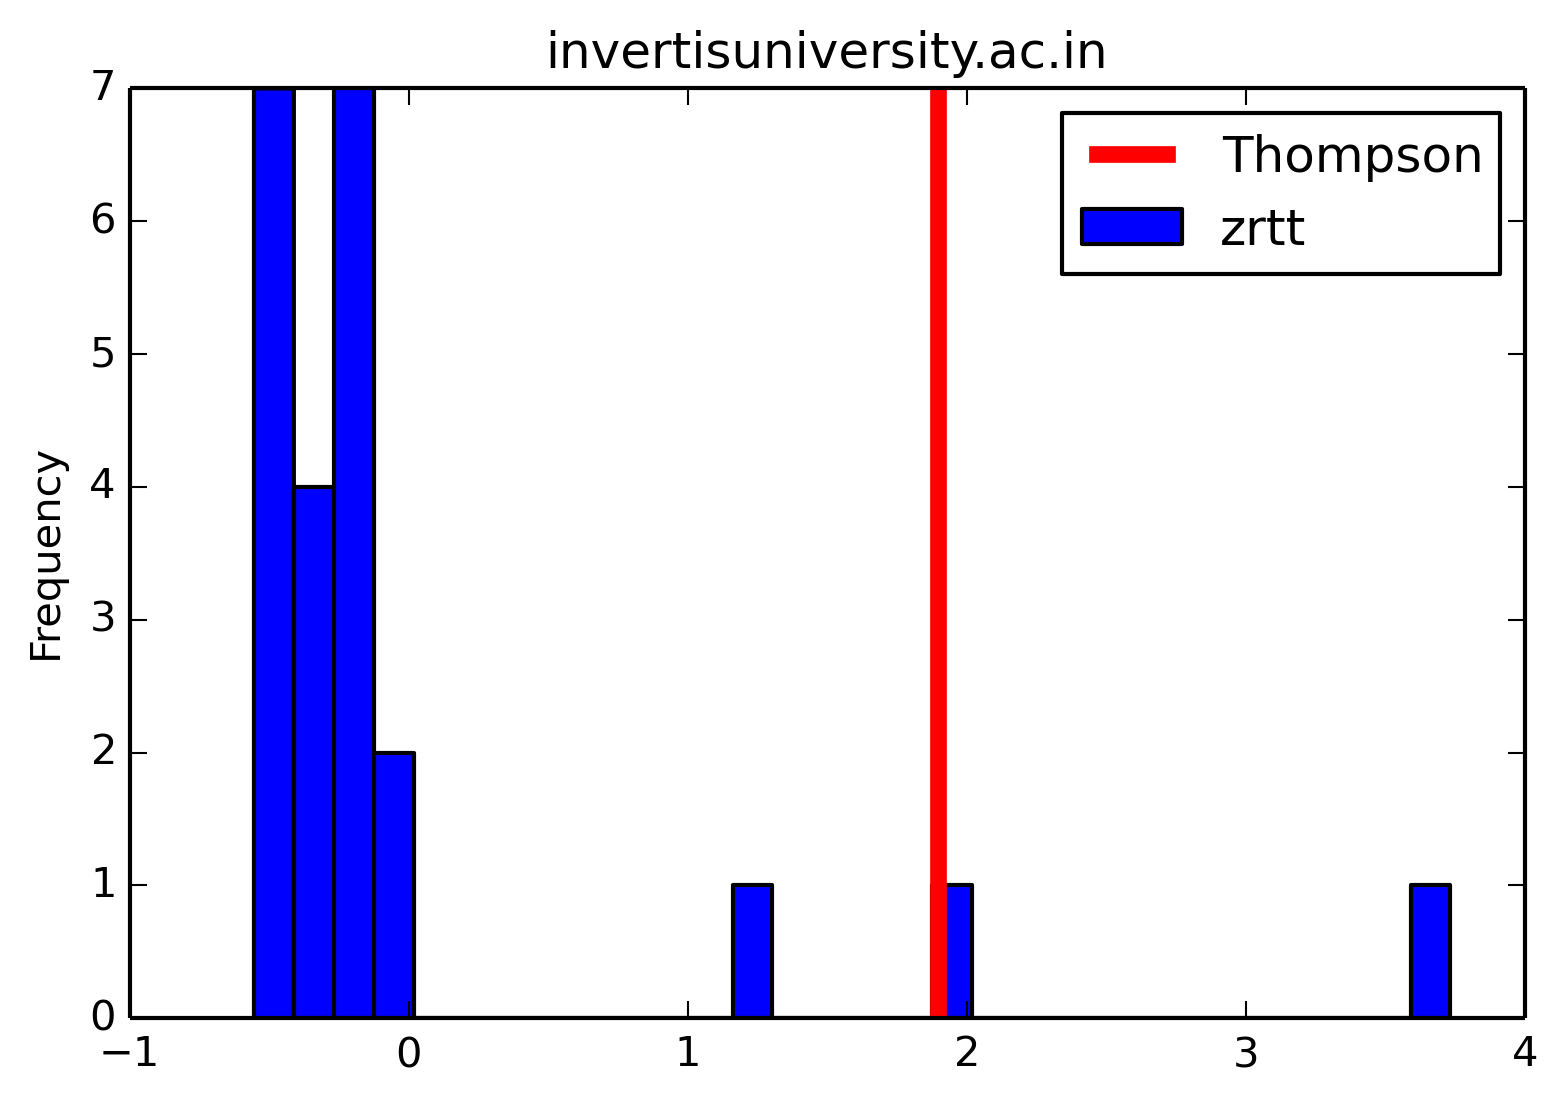
\includegraphics[width=0.45\textwidth]{histogramas_thompson/invertisuniversity-ac-in.png}
  \caption{RTTs Normalizados comparados con el valor Thompson}
  \label{entropia-s}
\end{figure}

\begin{figure}[H]
  \centering
    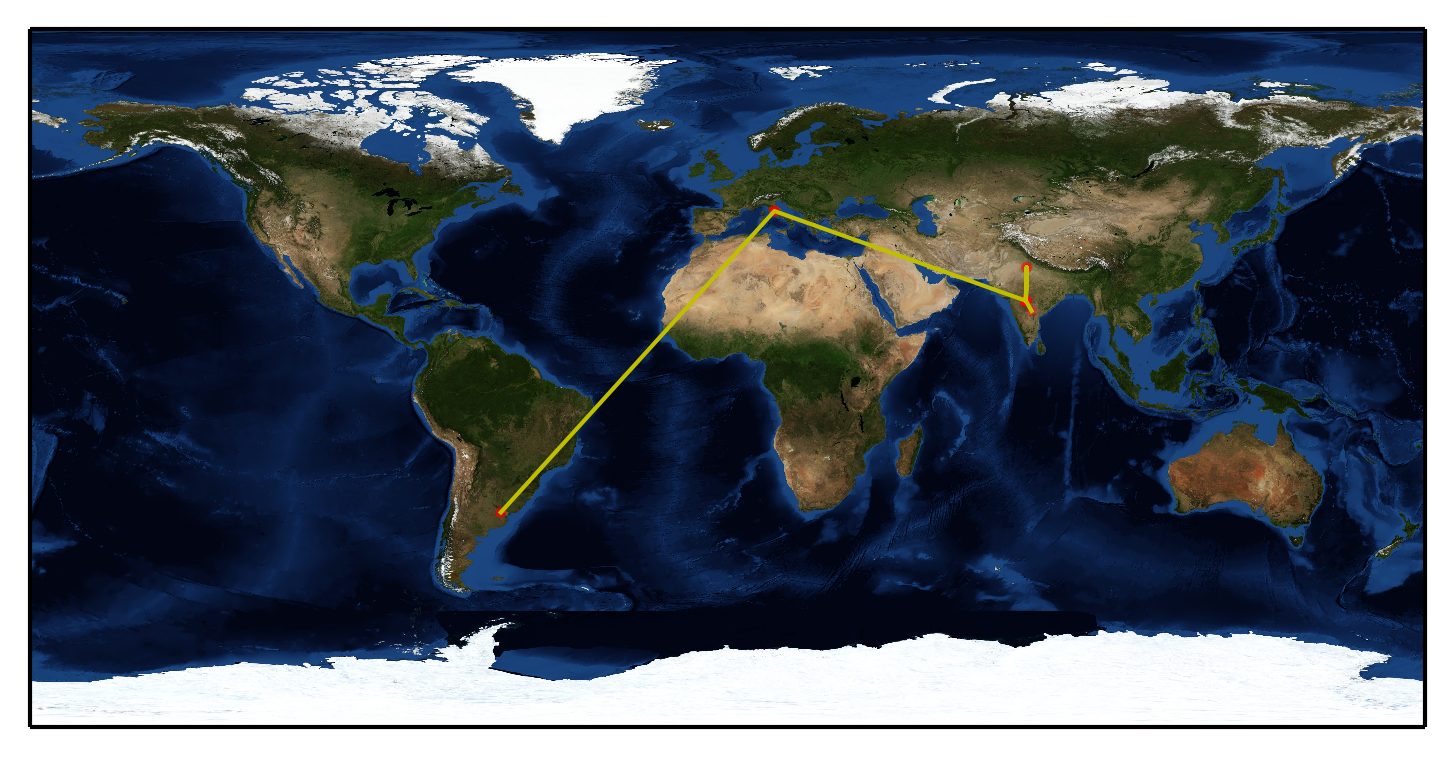
\includegraphics[width=0.45\textwidth]{grafico-rutas/invertisuniversity-ac-in.png}
  \caption{Gráfico de la ruta}
  \label{entropia-s}
\end{figure}




\subsection{Servidor www.uae.ma}
\begin{figure}[H]
  \centering
    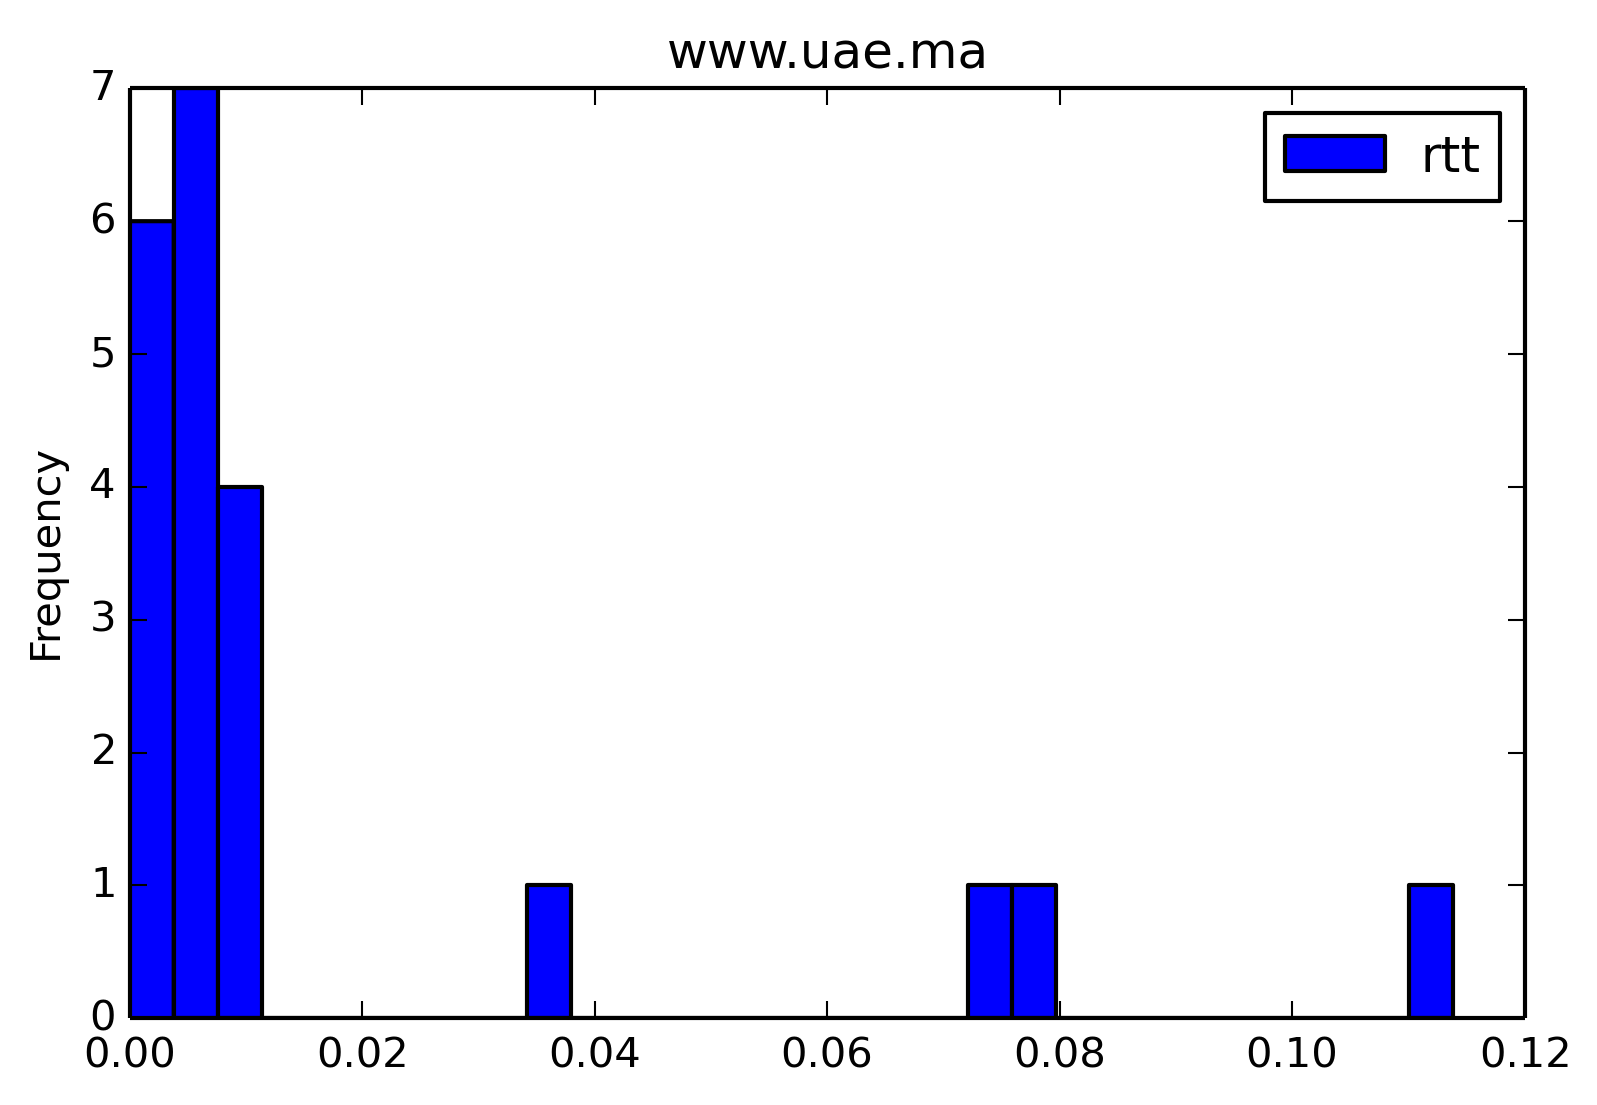
\includegraphics[width=0.45\textwidth]{histogramas_rtt/www-uae-ma.png}
  \caption{RTT entre saltos}
  \label{entropia-s}
\end{figure}

\begin{figure}[H]
  \centering
    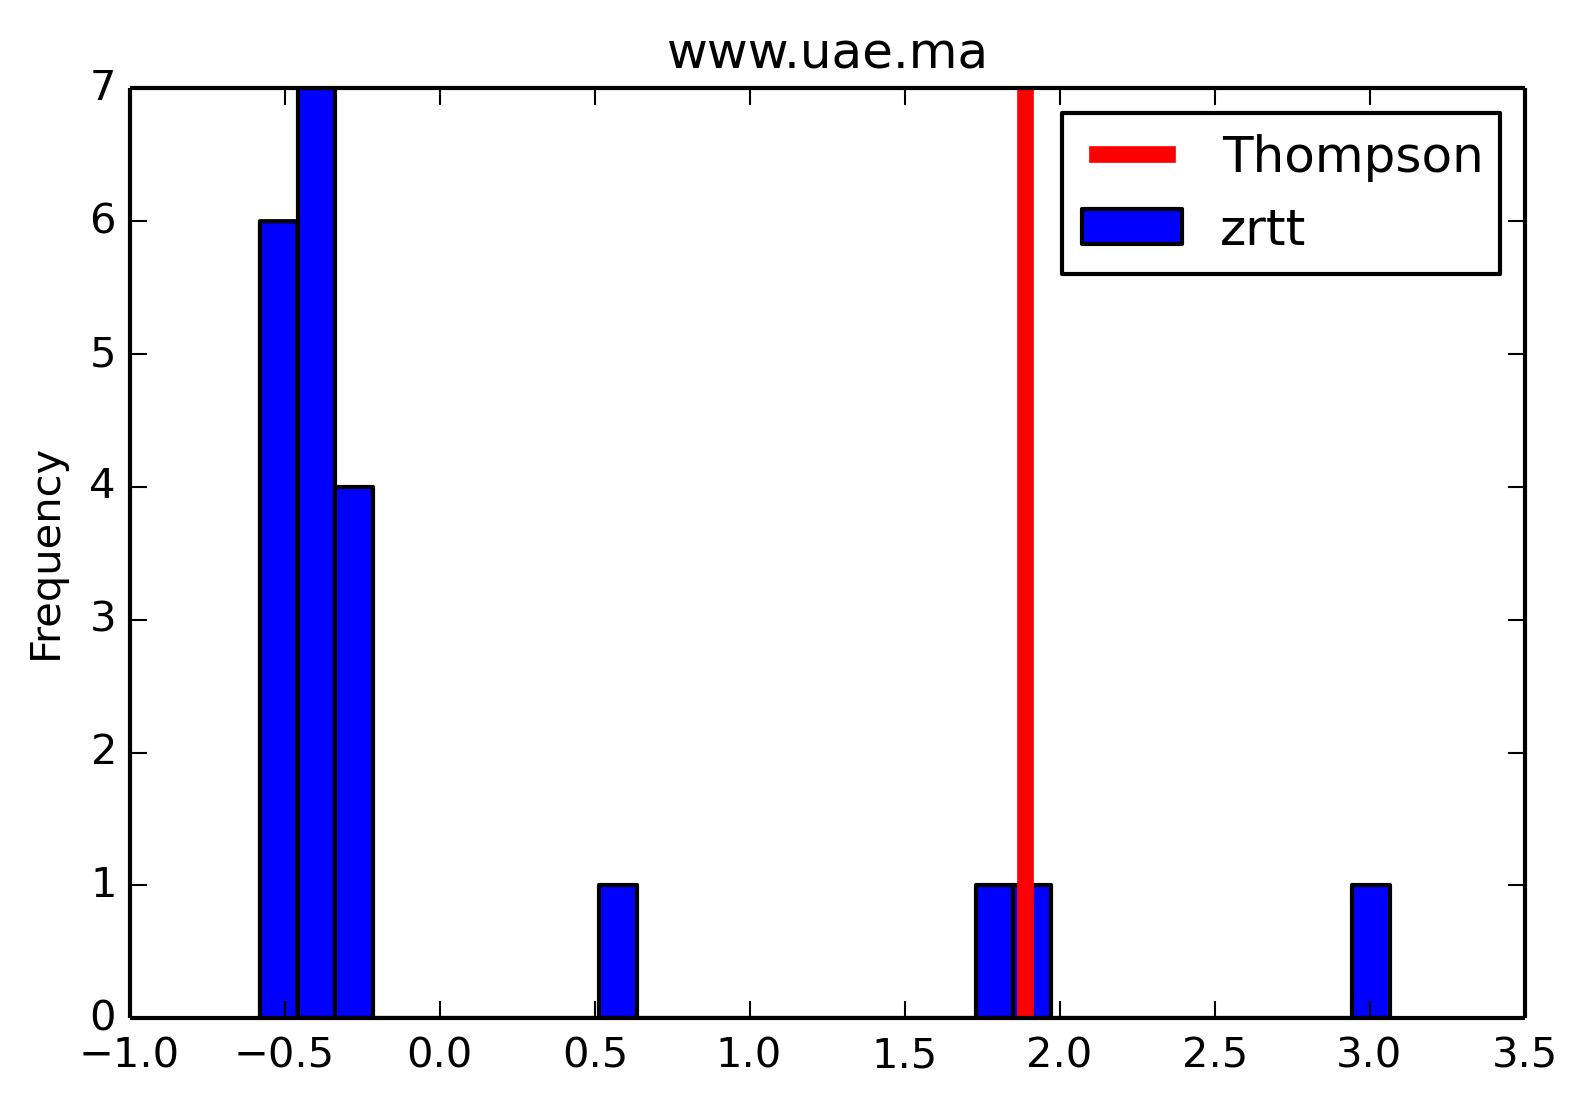
\includegraphics[width=0.45\textwidth]{histogramas_thompson/www-uae-ma.png}
  \caption{RTTs Normalizados comparados con el valor Thompson}
  \label{entropia-s}
\end{figure}

\begin{figure}[H]
  \centering
    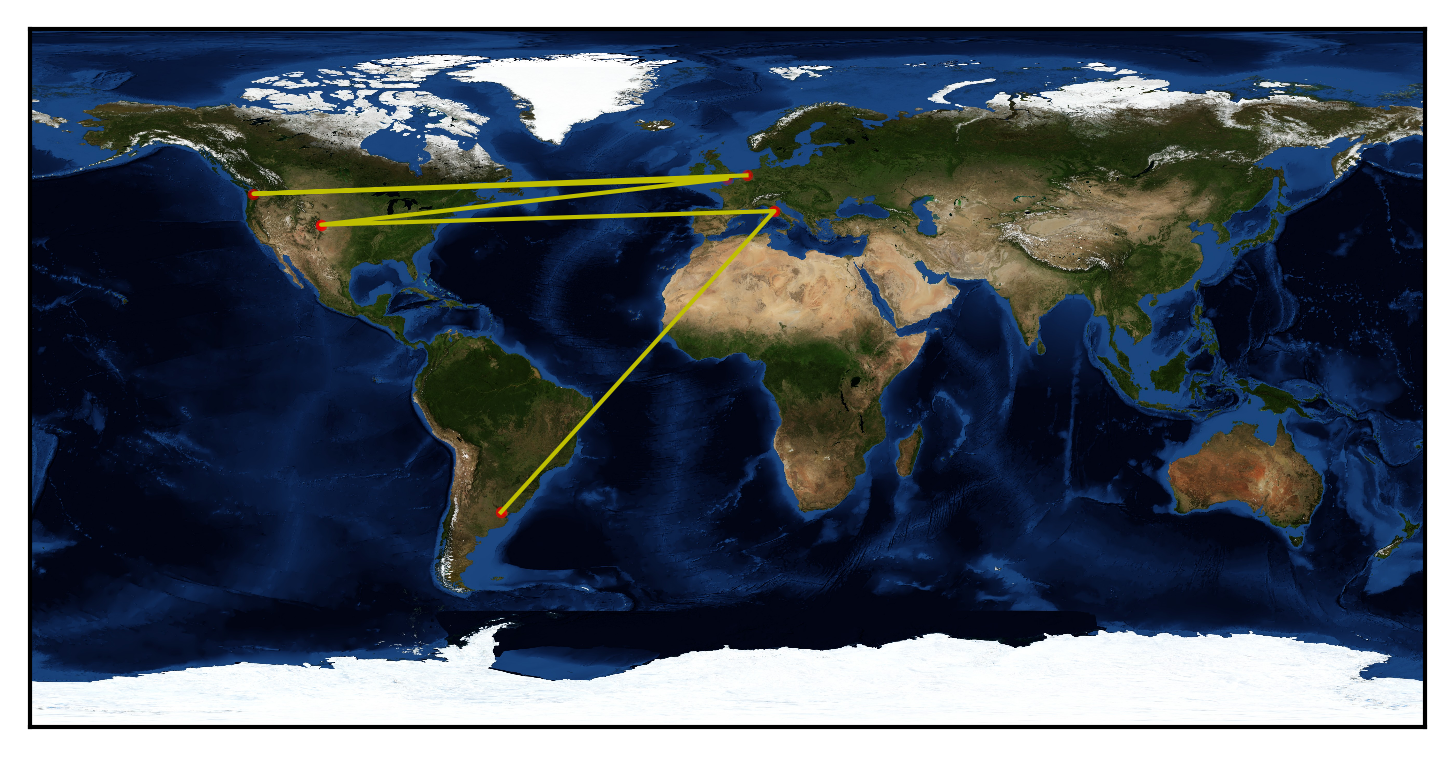
\includegraphics[width=0.45\textwidth]{grafico-rutas/www-uae-ma.png}
  \caption{Gráfico de la ruta}
  \label{entropia-s}
\end{figure}




\subsection{Servidor bifrost.is}
\begin{figure}[H]
  \centering
    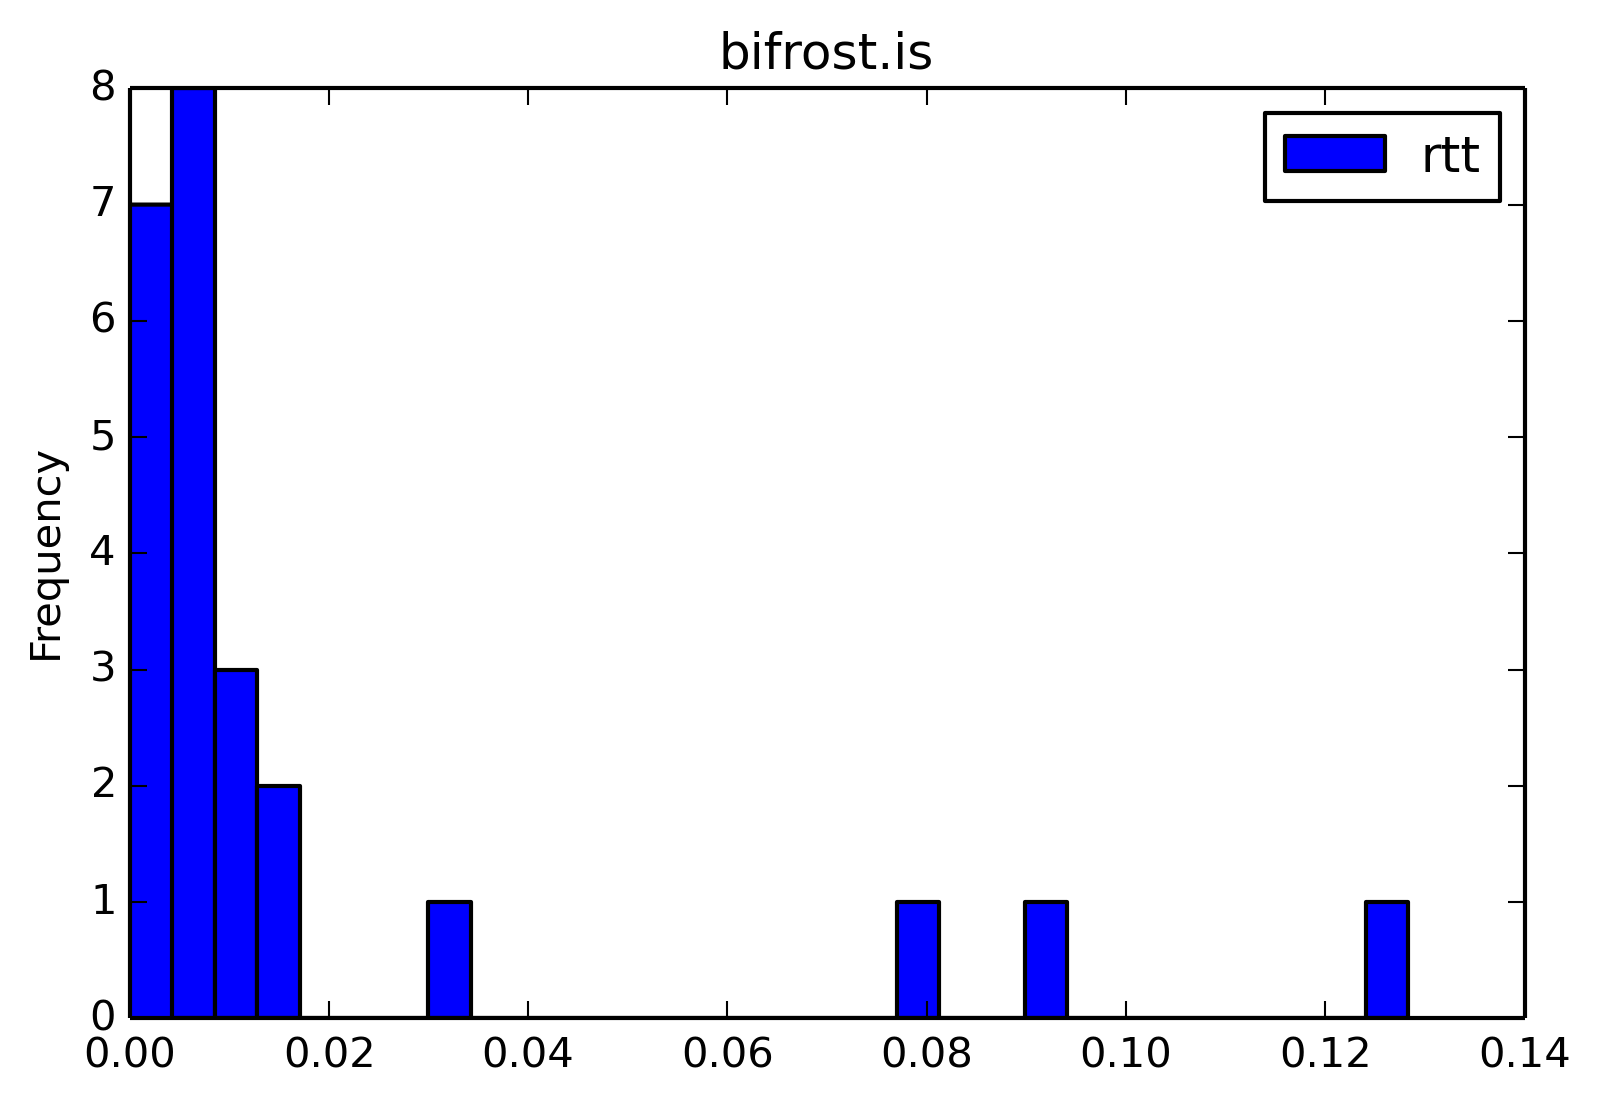
\includegraphics[width=0.45\textwidth]{histogramas_rtt/bifrost-is.png}
  \caption{RTT entre saltos}
  \label{entropia-s}
\end{figure}

\begin{figure}[H]
  \centering
    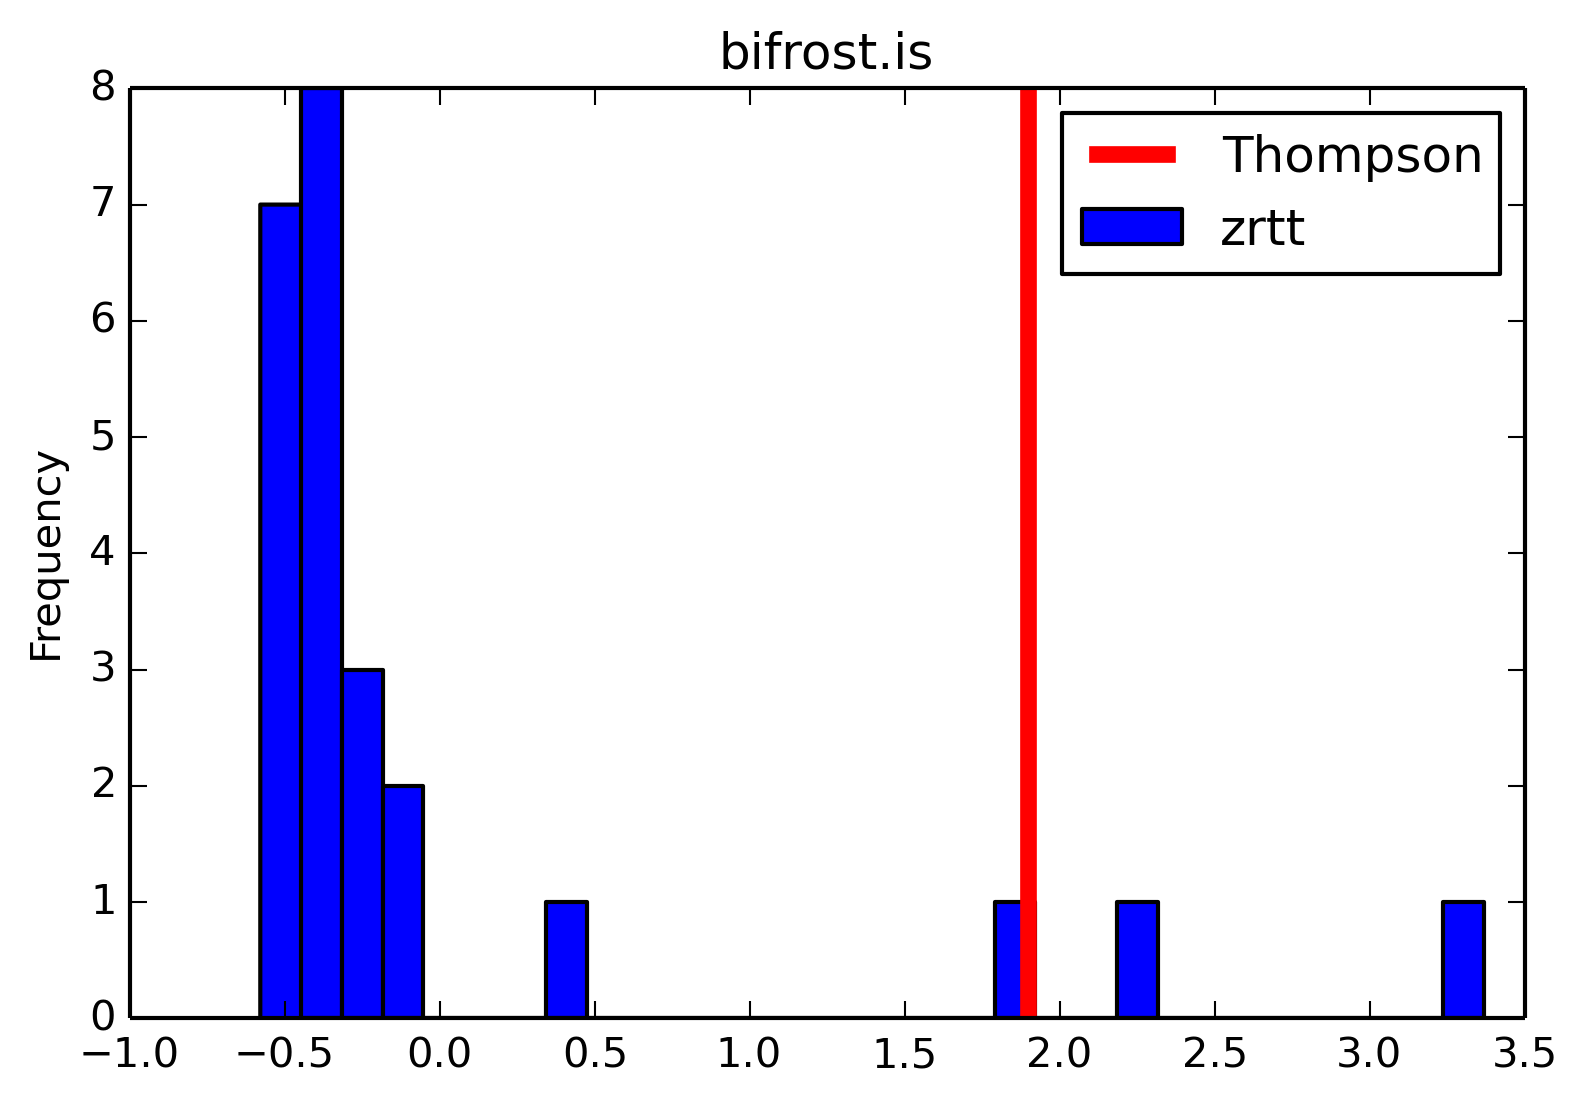
\includegraphics[width=0.45\textwidth]{histogramas_thompson/bifrost-is.png}
  \caption{RTTs Normalizados comparados con el valor Thompson}
  \label{entropia-s}
\end{figure}

\begin{figure}[H]
  \centering
    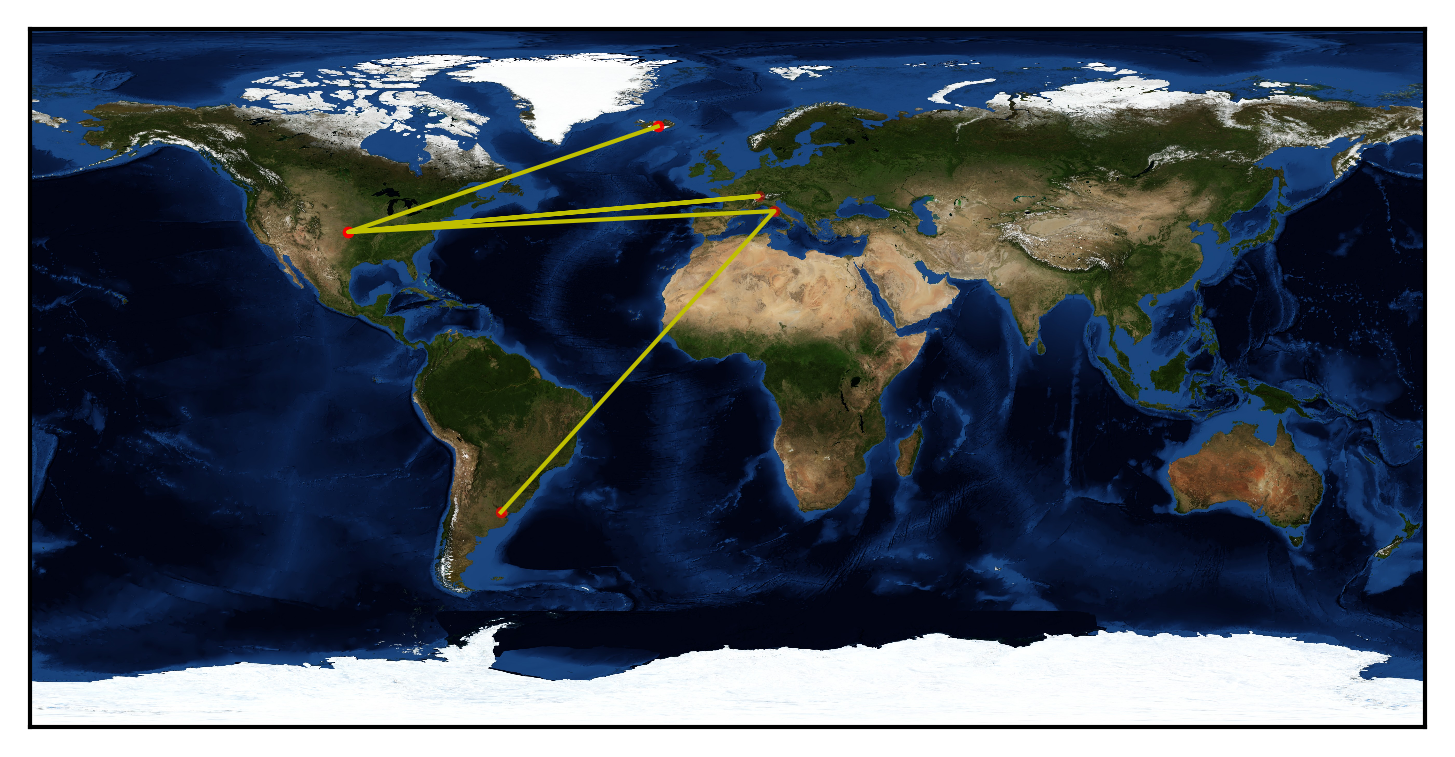
\includegraphics[width=0.45\textwidth]{grafico-rutas/bifrost-is.png}
  \caption{Gráfico de la ruta}
  \label{entropia-s}
\end{figure}




\subsection{Servidor birmingham.ac.uk}
\begin{figure}[H]
  \centering
    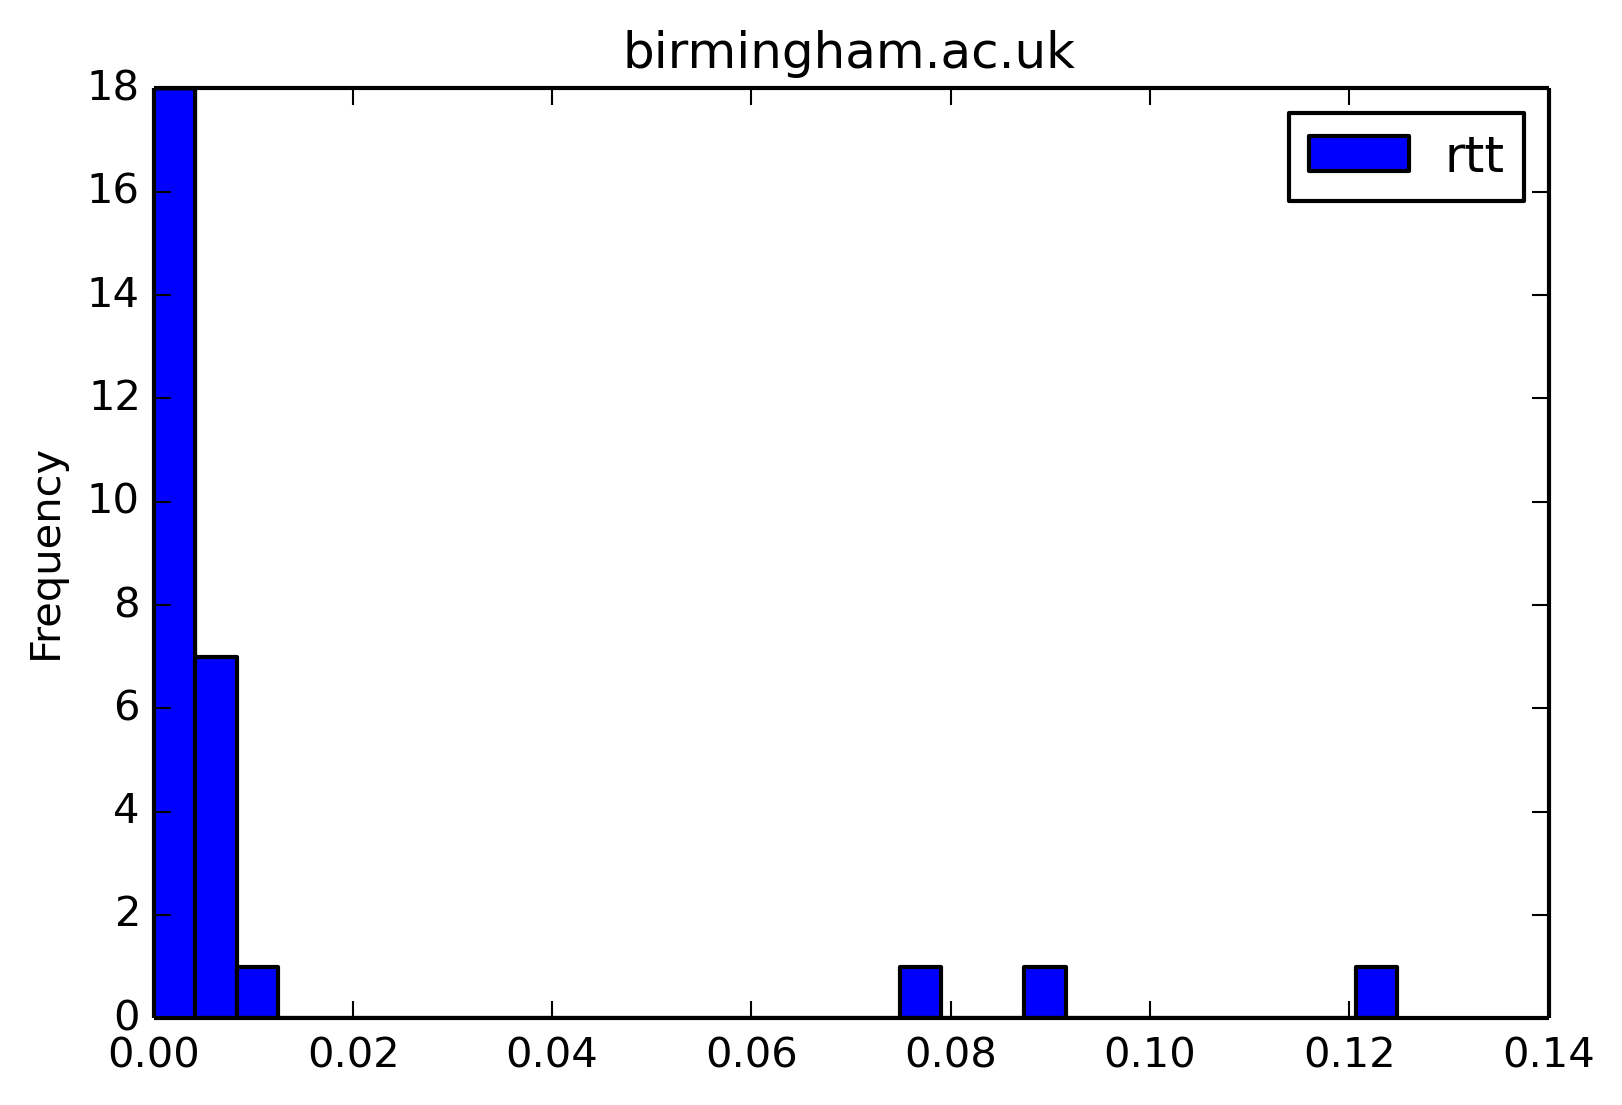
\includegraphics[width=0.45\textwidth]{histogramas_rtt/birmingham-ac-uk.png}
  \caption{RTT entre saltos}
  \label{entropia-s}
\end{figure}

\begin{figure}[H]
  \centering
    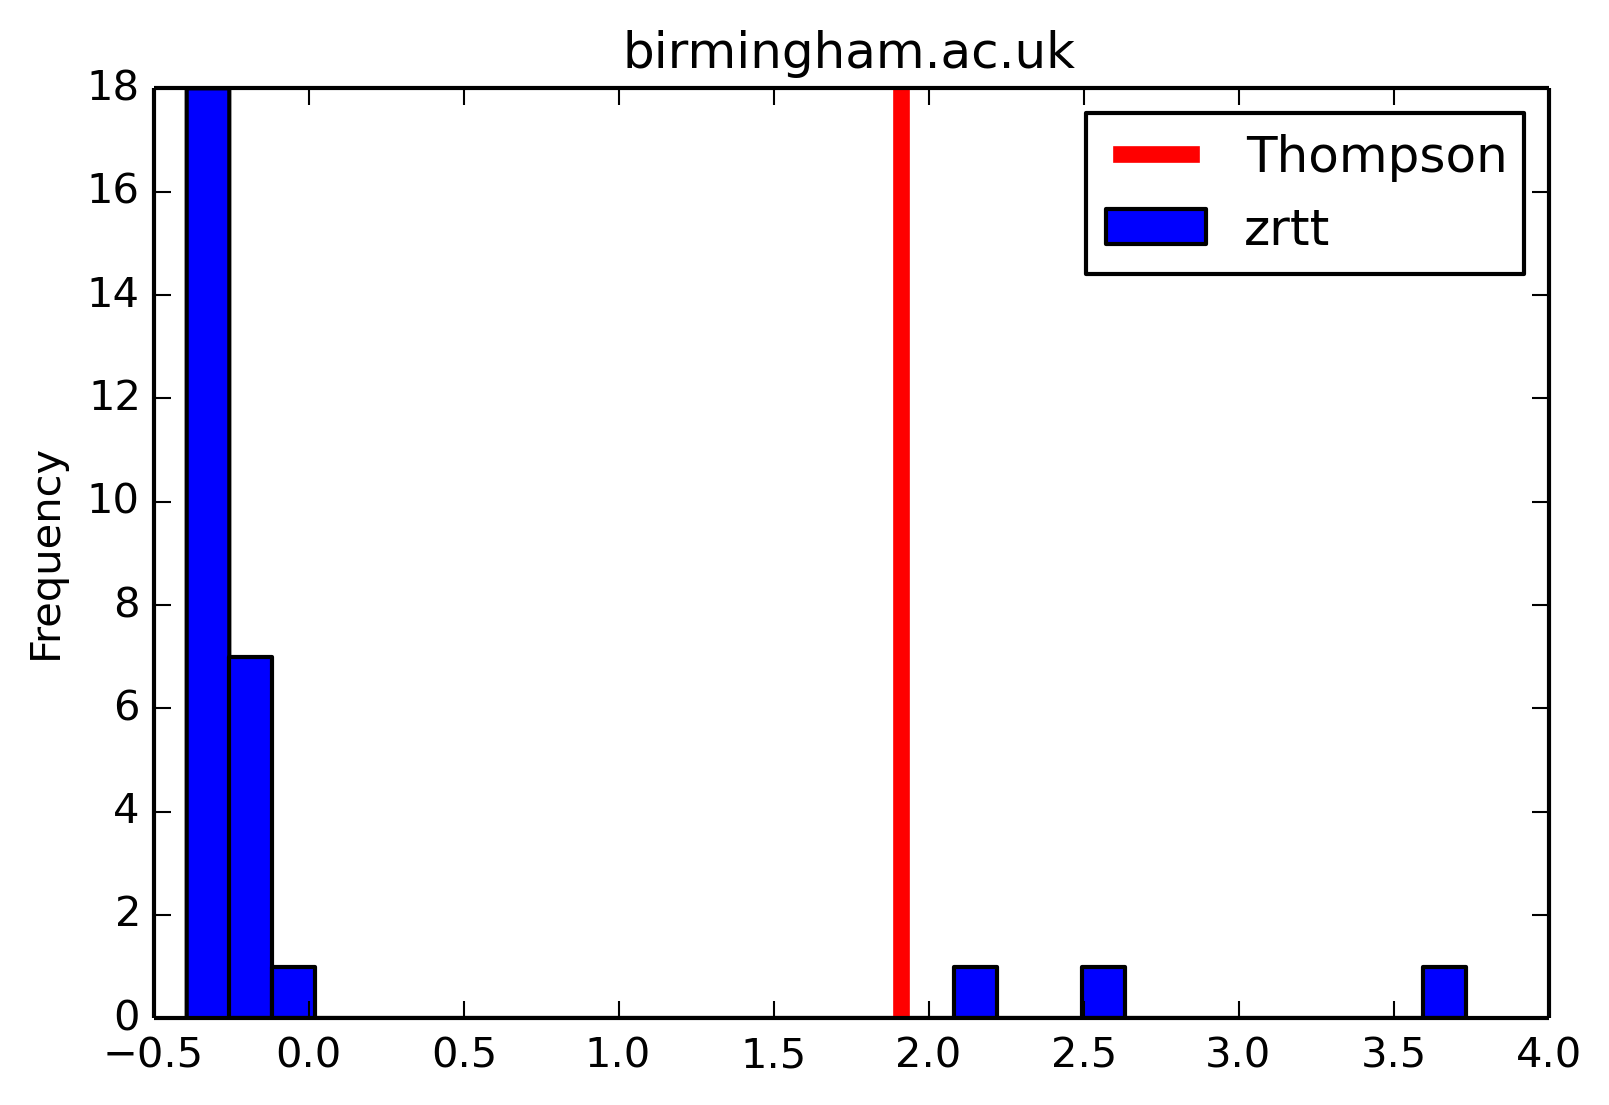
\includegraphics[width=0.45\textwidth]{histogramas_thompson/birmingham-ac-uk.png}
  \caption{RTTs Normalizados comparados con el valor Thompson}
  \label{entropia-s}
\end{figure}

\begin{figure}[H]
  \centering
    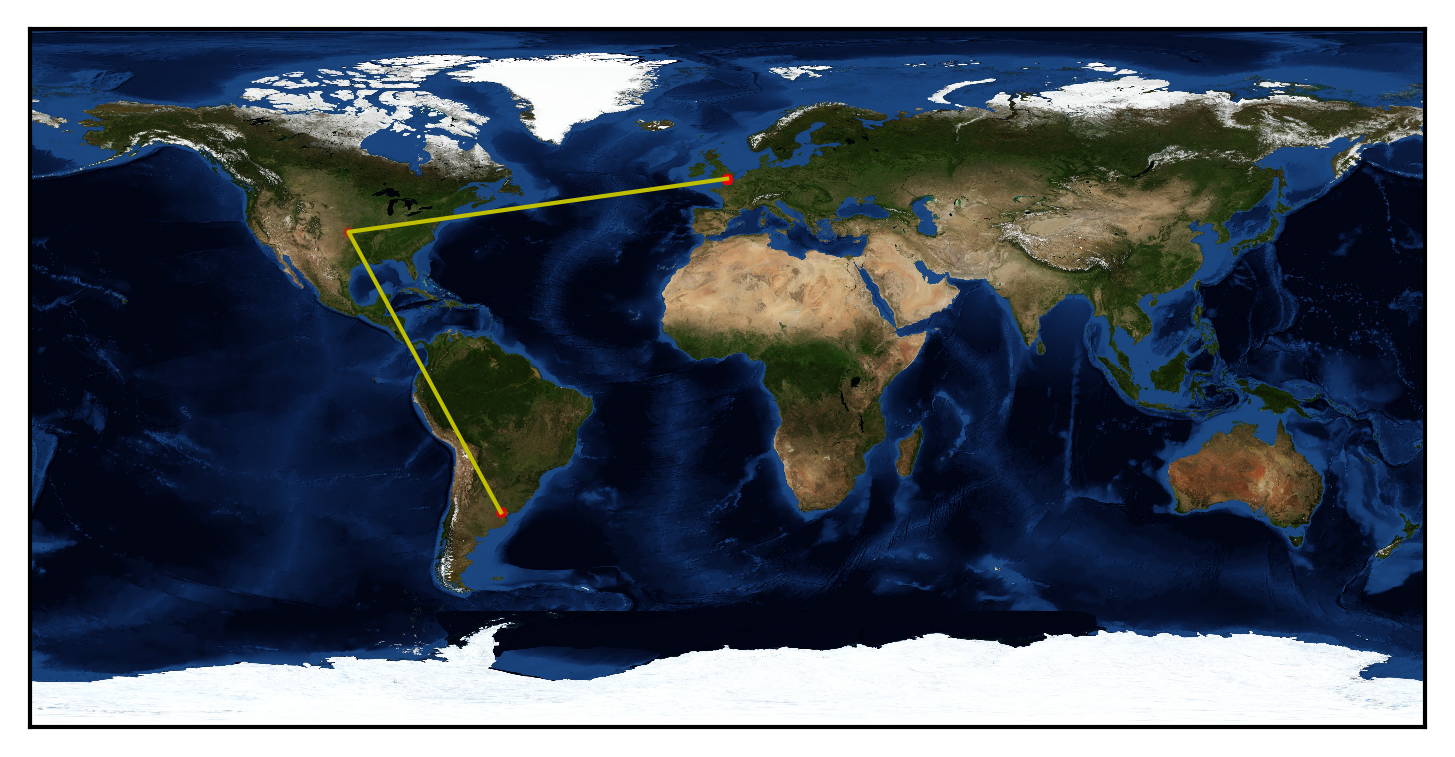
\includegraphics[width=0.45\textwidth]{grafico-rutas/birmingham-ac-uk.png}
  \caption{Gráfico de la ruta}
  \label{entropia-s}
\end{figure}